\documentclass[a4paper,11pt,twoside,openright]{memoir}

% pacchetti e definizioni
\usepackage[utf8]{inputenc}
\usepackage[english]{babel}
\usepackage{amsmath}
\usepackage{amssymb}
\usepackage{amsthm}
\usepackage{commath}
\usepackage{mathtools}
\usepackage{faktor}
\usepackage{color}
\usepackage{graphicx}
\usepackage{multirow}
\usepackage{array}
\usepackage{multirow}
\usepackage{breqn}
\usepackage[adversary, operators, sets, primitives, notions, probability, advantage, ff]{cryptocode}
\usepackage{todonotes}
\usepackage{tikz-cd}
\usepackage{hyperref}

\hypersetup{
    colorlinks,
    citecolor=black,
    %filecolor=black,
    linkcolor=black,
    urlcolor=blue
}

%\addtolength{\topmargin}{-.5in}
%\addtolength{\textheight}{0.5in}



\newtheorem{theorem}{Theorem}[section]
\newtheorem*{theorem*}{Theorem}
%\newtheorem{algorithm}[theorem]{Algoritmo}
%\newtheorem{claim}[theorem]{Claim}
%\newtheorem{conjecture}[theorem]{Congettura}
\newtheorem{corollary}[theorem]{Corollary}
\newtheorem{lemma}[theorem]{Lemma}
\newtheorem{problem}{Problem}[section]
\newtheorem{proposition}[theorem]{Proposition}

\theoremstyle{definition}
\newtheorem{definition}{Definition}[section]
\newtheorem{example}[theorem]{Example}

\theoremstyle{remark}
\newtheorem*{remark}{Remark}
\newtheorem{assumption}{Assumption}[section]
\newtheorem*{oss}{Observation}



\newcommand{\zdv}{\adversary{Z}}
\newcommand{\Fun}{\mathcal{F}}
\newcommand{\keygen}{\mathsf{KeyGen}}
\newcommand{\encaps}{\mathsf{Encaps}}
\newcommand{\decaps}{\mathsf{Decaps}}


\DeclareMathOperator{\lcm}{lcm}
\DeclareMathOperator{\Imm}{Im}
\DeclareMathOperator{\Dom}{Dom}
\DeclareMathOperator{\End}{End}
\DeclareMathOperator{\Hom}{Hom}
\DeclareMathOperator{\Aut}{Aut}
\DeclareMathOperator{\car}{char}
\DeclareMathOperator{\st}{\; |\;}
\DeclareMathOperator{\et}{\;\wedge\;}
\DeclareMathOperator{\tr}{Tr}
\DeclareMathOperator{\n}{N}
\DeclareMathOperator{\disc}{disc}
\DeclareMathOperator{\GL}{GL}


\newcommand{\N}{\mathbb{N}}
\newcommand{\Z}{\mathbb{Z}}
\newcommand{\Q}{\mathbb{Q}}
\newcommand{\R}{\mathbb{R}}
\newcommand{\C}{\mathbb{C}}
\newcommand{\F}{\mathbb{F}}
\newcommand{\Oc}{\mathcal{O}}
\newcommand{\Zn}[1]{\Z/#1\Z}
\newcommand{\ds}{\displaystyle}
\newcommand{\eps}{\varepsilon}


%\chapterstyle{madsen}
%\chapterstyle{crosshead}
%\chapterstyle{veelo}
\chapterstyle{ell}



\checkandfixthelayout

\setlength{\parindent}{0pt}
%\nonzeroparskip
\setlength{\parskip}{4pt}
\setulmarginsandblock{3.5cm}{*}{1.3}
\setlrmarginsandblock{3cm}{*}{1.2}
\checkandfixthelayout


\newtheorem{theorem}{Theorem}[section]
\newtheorem*{theorem*}{Theorem}
\newtheorem{corollary}[theorem]{Corollary}
\newtheorem{lemma}[theorem]{Lemma}
\newtheorem{proposition}[theorem]{Proposition}
\newtheorem{problem}{Problem}[section]
\newtheorem{claim}[problem]{Claim}

\theoremstyle{definition}
\newtheorem{definition}[theorem]{Definition}
\newtheorem{example}[theorem]{Example}

\theoremstyle{remark}
\newtheorem*{remark}{Remark}
\newtheorem*{oss}{Observation}
\newtheorem{assumption}[problem]{Assumption}


\hypersetup{
    colorlinks,
    citecolor=black,
    %filecolor=black,
    linkcolor=black,
    urlcolor=blue
}



\begin{document}
\makeevenfoot{ruled}{}{\thepage}{}
\makeoddfoot{ruled}{}{\thepage}{}
\pagestyle{ruled}

\createprocedureblock{myproc}{center, boxed}{}{}{}


\frontmatter
\advance\vsize by 2.5cm % Advance page height
\advance\voffset by -1.5cm % Shift top margin


\begin{titlingpage}


\advance\hsize by 2.7cm % Advance page height
\advance\hoffset by -1.35cm % Shift top margin


%%\aliaspagestyle{titlingpage}{empty}

%\newgeometry{margin=2.5cm}

\calccentering{\unitlength}
\begin{adjustwidth*}{\unitlength}{-\unitlength}


\thispagestyle{empty}
\begin{center}
\large
\textsc{\Large Università di Pisa\\}
\vspace{0.6cm}

\includegraphics[width=3.8cm]{cherubino.pdf}

\vspace{0.8cm}
\textsc{\Large{Facoltà di Matematica}}\\



\vspace{2.5cm}


{\Huge\textbf{Isogeny-based Oblivious Transfer Protocols}}
\\[2.0cm]

\textsc{Tesi di Laurea Magistrale \\[0.2cm] in Matematica}\\
\vspace{0.5cm}

\begin{center}

%\textsc{\Large Anno Accademico 2010/2011}
\end{center}

\vspace{0.2cm}

\begin{center}
\makebox[\textwidth]{
\begin{tabular}{l p{5.3cm} r}
\textsc{{\LARGE Candidato}} & & \textsc{{\LARGE Relatore}} \\
\textbf{{\small Riccardo Zanotto}} & & {\small\textbf{Prof.ssa Emmanuela Orsini}} \\
  & & {\small COSIC, KU Leuven} \\
\end{tabular}}
\end{center}




\vspace{4.8cm}


\textsc{Anno Accademico 2020 - 2021}\\[0.2cm]


\end{center}

\end{adjustwidth*}


\advance\hsize by -2.7cm % Advance page height
\advance\hoffset by 1.35cm % Shift top margin


\end{titlingpage}


\advance\vsize by -2.5cm % Return old margings and page height
\advance\voffset by 1.5cm % Return old margings and page height



%\par\vfill\break % Break the page with different margins



%\restoregeometry


\thispagestyle{empty}
\null\vspace {\stretch {1}}
\begin{flushright}
    \textit{A nonna Gina}
\end{flushright}
\vspace {\stretch {2}}\null

\cleardoublepage


\tableofcontents


\mainmatter
\chapter*{Introduction}
\addcontentsline{toc}{chapter}{Introduction}

The main goal of this thesis is to study isogeny-based cryptography, and some proposed oblivious transfer protocols based on it, with particular attention to security properties and proofs.

Oblivious transfer is one of the most basic functionalities between two parties, and has been introduced by Rabin \cite{Rabin_OT} as one of the earliest examples of multi-party computation; MPC is the sub-field of cryptography that studies methods for multiple parties to be able to compute some public function, while keeping the inputs private. For example, the function might be ``the sum of all inputs" or ``who won the election?".

In the case of oblivious transfer the function is $f((m_0,m_1),\sigma)=(\lambda,m_\sigma)$, where $\lambda$ is the empty string, meaning that the first party doesn't receive any output. The importance of OT is that it can be composed to get any arbitrary secure function evaluation \cite{GMW}; it is then of great importance to study the most efficient and secure ways to realize OT.

There are many OT protocols which are based on the classical cryptography problems like RSA, Diffie-Hellman or ECDH. However, since all these problems become ``easy" with access to a quantum computer, in the recent years there has been a great effort in producing new cryptographic primitives that are quantum resistant.

The National Institute of Standards and Technology (NIST) has started in 2016 a competition to find a new post-quantum secure standard algorithm for KEMs and digital signatures. We are currently at round 3, with 4 KEM and 3 signature algorithms left, and some more ``alternate" algorithms.

The main areas from which the finalists and the alternate protocols have been drawn are the following:
\begin{itemize}
    \item Coding theory
    \item Lattice theory
    \item Multivariate equations
    \item Hash functions
    \item Supersingular isogenies
\end{itemize}

Beyond the NIST competition, also the MPC world is trying to adopt some post-quantum constructions for its protocols. The most promising one, both for the NIST competition and the MPC protocols, is probably lattice-based cryptography, from which OT protocols have already been constructed \cite{PVW}. However, we will focus on isogeny-based cryptography, which is a pretty new sub-field.

The main idea of isogeny crypto is to use graphs of elliptic curves, where the nodes are supersingular $j$-invariants and the edges are isogenies between them. The reason why this is useful for cryptography is that it's easy to compute a random isogeny from a given curve (i.e. a walk in the graph), but it's hard to find an isogeny given two different curves.

Isogeny-based cryptography has two main constructions, which are SIDH \cite{SIDH11} and CSIDH \cite{CSIDH}. They both are key exchange algorithms, but they are quite different: SIDH works on a graph defined over $\F_{p^2}$, while CSIDH is over $\F_p$ and uses the action of the class group on elliptic curves.

After introducing isogeny crypto with its assumptions and constructions, we will analyze how to build OT protocols based on it. Our focus will be provable security of those protocols, i.e. against what attacks they are secure and if they can be composed to make MPC protocols.

In general defining the security of a MPC protocol is much more challenging than defining security for an encryption scheme; for the latter we have the usual game-based definitions, while for complex protocols we need something more. In particular, we will need simulation-based security notions.

The most used framework in which to prove security is called Universal Composability: its aim is to model any generic computation, with any security guarantee. At the heart of the framework is the following idea: we distinguish the \emph{real world} in which the protocol is actually executed, and the \emph{ideal world} in which the parties interact with a trusted third party. We program the trusted party with the computation we want to do and say that the protocol securely implements the computation if any attacker in the real world can be simulated in the ideal world.

This means that any attacker cannot really gain more information apart from what we let it know in the ideal functionality. In the case of a distributed function evaluation, the trusted party will collect all the inputs and then deliver all the outputs to the specified parties; so UC is a formalization of the security statement ``an attacker cannot learn anything apart from the output of the function".

As with classical definitions of security, we can model different types of adversaries. In UC, the main distinction is between \emph{semi-honest} and \emph{malicious}; the first type actually follows the protocol and is only trying to get more information, and is useful for modeling \emph{colluding} parties that try to obtain knowledge of the other parties' inputs; a malicious adversary can instead send arbitrary messages and in some cases can disrupt the protocol denying the delivery of the output to the honest parties.

Another feature of UC is the hybrid world, in which a protocol is executed in the real world, but has access to some other ideal functionality; in this way we can decide to work in the \emph{plain model} or to admit \emph{random oracles} and trusted setups. Moreover, by changing the model of computation, we can impose some behaviour on the parties and the adversary.

We will then analyze OT protocols using the UC framework; in particular, we first study the ``simplest OT" by Chou and Orlandi \cite{Chou_Orlandi}, which is based on the usual elliptic curve Diffie-Hellman. This is an important protocol, not only because it is very efficient, but also because its UC-security proof contains some errors.

The issues of the proof are not limited to that protocol, but the underlying motivations (in particular the input extraction of the choice bit from a corrupted receiver) impose strict constraints in the design of OT protocols; this means that usually they require additional computations and rounds just to be able to conclude the UC-security proof, for a very technical reason and not because they are actually insecure. This greatly reduces their efficiency, while for fast MPC we need very fast OT protocols.

A possible remedy for the Chou and Orlandi protocol comes from the \emph{Algebraic Group Model}, which makes all the machines give a representation for every group element that they output. In \cite{AGM_UC} it is explained how the AGM allows for a complete proof of UC-security against malicious adversaries for the ``simplest OT", since they use the elements' representation to extract the choice bit.

In the last chapter we will briefly overview some OT constructions based on isogenies, and then will focus on the protocol proposed in \cite{Lai_twists}. The core of the protocol has two rounds and is UC-secure against semi-honest adversaries; however, to achieve security against malicious adversaries the authors need to introduce a third round of communication that serves as a ``proof of decryption" and is used for the input extraction.

Finally, inspired by the effectiveness of AGM for the Chou and Orlandi protocol, we introduce a new computational model, which we call \emph{Explicit Isogenies} (EI), meaning that instead of giving a representation for a group element, the adversary has to ``explain" each curve $E$ that it outputs by giving an isogeny $\phi:E_i\to E$ from a known curve $E_i$.

Our EI model, in the CSIDH setting, will allow us to prove security for the two-round version of Lai et al. protocol. This is a very interesting result, since there is some evidence that the EI model might actually be equivalent to the plain model of UC.

The problem to which the expressiveness of our EI model reduces is the one of \emph{sampling} random supersingular curves. It is one of the open problems in isogeny-based cryptography, and one that is starting to be believed difficult.

The main result of this thesis is the introduction of the EI model, which allows to prove UC-security for efficient OT protocols, without having to worry too much about input extraction. Moreover, if the sampling problem is hard, we claim that our EI model is equivalent to the full UC model.


\part{Background}
\chapter{Mathematical background}

The theory of elliptic curves is at the foundation of isogeny-based Cryptography, but in a very different style from classical Elliptic Curve Cryptography: the latter uses the group of points of a single curve, while the first uses graphs of elliptic curves.

Our introduction on these topics will follow \cite{Silverman} and \cite{DeFeo_intro}.

\section{Elliptic curves}

We start by giving the most general definition of an elliptic curve over a field $K$.

\begin{definition}
    An \emph{elliptic curve} $E$ \emph{over} $K$ is a smooth projective curve of genus $1$, with a given $K$-rational point.
\end{definition}

Since we will work over finite fields of large characteristic, we will assume in all our theorems that $\car K\neq 2,3$. This allows us to simplify the representation of an elliptic curve.

\begin{proposition}[Weierstrass model]
    Let $E$ be an elliptic curve over $K$, with $\car K\neq 2,3$. Then $E$ is isomorphic to the curve $$ZY^2=X^3+aXZ^2+bZ^2$$ with $a,b\in K$ and $4a^3+27b^2\neq0$.
    
    The point $O=(0:1:0)$ is called the \emph{point at infinity} of $E$, and it's the only point on $Z=0$.
\end{proposition}

Usually we then identify the curve with its affine patch at $Z\neq0$, i.e. with the equation $$y^2=x^3+ax+b,$$
plus the point at infinity $O$.

Any elliptic curve can (almost) be identified by a single number, the \emph{$j$-invariant}:
\begin{theorem}
    Let $E:y^2=x^3+ax+b$ an elliptic curve over $K$, and let its $j$-invariant be $$j(E)=1728\frac{4a^3}{4a^3+27b^2}.$$
    
    Then any other curve $E'$ is isomoprhic to $E$, over $\bar K$, if and only if $j(E)=j(E')$.
\end{theorem}

We will make precise sense of what ``almost" and ``isomorphic" means in the next sections when we will introduce isogenies and twists.

Elliptic curves are also well known for naturally having a structure of abelian group, with the point at infinity $O$ as the neutral element.

\begin{theorem}
    Let $E$ an elliptic curve over $K$, given by a Weierstrass equation $y^2=x^3+ax+b$. Then there exists an abelian group law $\oplus$ on the set of $L$-rational points $E(L)$ for any field extension $K\subset L$.
    
    Given affine points $P_1=(x_1,y_1)$ and $P_2=(x_2,y_2)$ the addition law is defined by:
    \begin{itemize}
        \item If $x_1=x_2$ and $y_1=-y_2$, then $P_1\oplus P_2=O$.
        \item Otherwise $P_1\oplus P_2=(x_3,y_3)$ with \begin{align*}
            x_3 &=  \lambda^2-x_1-x_2\\
            y_3 &= -\lambda x_3-y_1+\lambda x_1
        \end{align*}
        where $\lambda=\frac{3x_1^2+a}{2y_1}$ if $P_1=P_2$, and $\lambda=\frac{y_2-y_1}{x_2-x_1}$ otherwise.
    \end{itemize}
\end{theorem}\todo{maybe usual picture?}

The structure of this group has been much studied, and there are still open questions; luckily we will work in finite fields, where most of it is understood.

\begin{theorem}
    Let $E$ be an elliptic curve over an algebraically closed field $K$ of characteristic $p$, and let $m$ be an integer. Then the $m$-torsion group of $E(K)$, denoted by $E[m]$, is given by:
    \begin{itemize}
        \item $E[m]\cong \Zn{m}\times\Zn{m}$, if $p$ does not divide $m$.
        \item If $p>0$, then either $E[p^r]\cong\Zn{p^r}$ for all $r\ge0$ or $E[p^r]=\{O\}$.
    \end{itemize}
\end{theorem}

The curves where the last case happens are called \emph{supersingular}, and they are one of the main topics of this thesis.

\begin{theorem}
    Let $E$ be an elliptic curve over a field $K$. Then
    \begin{itemize}
        \item If $K$ is a number field, then $E(K)$ is a finitely generated abelian group.
        \item If $K=\F_q$, then $E(\F_q)\cong\Zn{n}\times\Zn{m}$, with $n\mid\gcd(m, q-1)$.
    \end{itemize}
\end{theorem}

The determination of the rank of $E(K)$ in the number field case is the focal point of the Birch and Swinnerton-Dyer conjecture, which is one of the Millennium Problems. It is also unknown if such rank is bounded or unbounded.

\section{Isogenies}

Since elliptic curves are algebraic varieties, we briefly recall some notions of maps between varieties.

\begin{definition}
    Let $V_1,V_2$ projective varieties over an algebraically closed field $\bar K$, and $\bar K(V_1), \bar K(V_2)$ their function fields.
    
    A \emph{rational map} $\phi:V_1\to V_2$ is $\phi=[f_1,\dots,f_n]$, where $f_i\in\bar K(V_1)$ such that for any point $P$ at which all $f_i$ are defined we have $\phi(P)=[f_1(P),\dots,f_n(P)]\in V_2$.
    
    A \emph{morphism} is a rational map that is regular at any point, i.e. for any $P\in V_1$ there exists a function $g\in\bar K(V_1)$ such that all $gf_i$ are defined at $P$, and at least one $gf_i(P)\neq0$.
\end{definition}
\todo{examples}

A very important property of morphisms is the following:
\begin{proposition}
    Let $\phi: V_1\to V_2$ a morphism of projective varieties defined over $K$, with $\phi=[f_1,\dots,f_n]$. Then the map $\phi^\ast:K(V_2)\to K(V_1)$ given by $\phi^\ast(g)(x)=g(f_1(x),\dots,f_n(x))$ is a homomorphism of $K$-algebras.
\end{proposition}

We now turn our attention to curves, which are varieties of dimension $1$, for example all polynomials $f(x,y)=0$ in two variables.

Since we will work over finite fields, it's important to clearly state the definition of separable and inseparable morphisms.

\begin{definition}
    Let $\phi:C_1\to C_2$ be a nonconstant morphism of curves defined over $K$. Then we define its \emph{degree} to be $$\deg\phi = [K(C_1):\phi^\ast K(C_2)].$$
    Moreover we say that $\phi$ is \emph{separable}, \emph{inseparable} or \emph{purely inseparable} exactly when the extension of function field is. Finally, we define $\deg_s\phi$ and $\deg_i\phi$ as the separable and inseparable degree of the field extension.
\end{definition}

A geometric interpretation of (separable) degree is the following, and in some sense it shows why it is the ``right" definition:

\begin{proposition}
    Let $\phi: C_1\to C_2$ be a morphism between smooth curves defined over $\bar K$. Then $\#\phi^{-1}(Q)=\deg_s\phi$ for all but finitely many $Q\in C_2$.
\end{proposition}

Turning back to elliptic curves, we are ready to define \emph{isogenies}.
\begin{definition}
    Let $E_1$ and $E_2$ be elliptic curves, with points at infinity $O_1,O_2$. An \emph{isogeny} is a morphism of curves $\phi:E_1\to E_2$ such that $\phi(O_1)=O_2$.
    
    We denote the set of isogenies from $E_1$ to $E_2$ by $\Hom(E_1, E_2)$.
\end{definition}

\begin{example}
    We set $E_1:y^2=x^3+x$ and $E_2:y^2=x^3-4x$. Then the map $\phi:E_1\to E_2$ defined by $$\phi(x,y)=\left(\frac{x^2+1}{x}, y\frac{x^2-1}{x^2}\right), \;\phi(0,0)=O$$ is a separable isogeny of curves over $\Q$. Its kernel has size $2$ and is generated by $(0,0)$.
    
    It is indeed a morphism, since in projective coordinates it can be written as
    \begin{align*}
    \phi(X:Y:Z) &= (X(X^2+Z^2):Y(X^2-Z^2):X^2Z)\\
    &= (Y(X^2+Z^2):XY^2-X^2Z-Z^3:XYZ)
    \end{align*}
    and is defined even at $(0:0:1)$.
\end{example}

Notice that $\Hom(E_1, E_2)$ is a group, with neutral element the constant isogeny that sends everything to $O_2$.

Moreover, the choice of the $\Hom$ notation is not random: it turns out that isogenies are the right morphisms for the category of elliptic curves, since we have the following:
\begin{proposition}
    Let $\phi:E_1 \to E_2$ be a nonconstant isogeny. Then $\phi$ induces a surjective group homomorphism $E_1(\bar K)\to E_2(\bar K)$ with finite kernel.
    
    In particular, $\#\ker \phi = \deg_s\phi = \#\phi^{-1}(Q)$ for \emph{any} $Q\in E_2(\bar K)$.
\end{proposition}

It turns out that the kernel of a separable isogeny completely determines it, and we have simple formulas to evaluate the resulting isogeny, due to Vélu.
\begin{proposition}
    Let $E$ be an elliptic curve over an algebraically closed field $\bar K$, and $G$ a subgroup of $E(\bar K)$. Then there is a curve $E'$ and a separable isogeny $\phi:E\to E'$ with $\ker\phi=G$; the curve and the isogeny are unique up to isomorphisms $E'\cong E''$.
    
    If $E$ is defined by the equation $y^2=x^3+ax+b$, then $E'$ has equation $y^2=x^3+a'x+b'$, where
    \begin{align*}
    a' &= a-5\sum_{Q\in G\setminus\{O\}}(3x(Q)^2+a)\\
    b' &= b-7\sum_{Q\in G\setminus\{O\}}(5x(Q)^2+3ax(Q)+2b)
    \end{align*}
    and for any $P\in E(\bar K)$ we have
    $$\phi(P) = \left(x(P) + \sum_{Q\in G\setminus\{O\}} x(P+Q)-x(Q), y(P)+ \sum_{Q\in G\setminus\{O\}} y(P+Q)-y(Q)\right)$$
\end{proposition}

Notice that, given these formulas, both the resulting curve and a point evaluation can be computed in $O(\# G)$ time.\todo{maybe explicit example}

One of the most important example of isogenies is multiplication-by-$m$:
\begin{example}
    For any $m\in\Z$ we have a natural isogeny $[m]:E\to E$, which we can define by induction with $[0](P)=O$, $[m+1]P=[m]P\oplus P$ and $[-m](P)=[m](-P)$. Since addition and negation are morphisms of curves, this actually defines an isogeny.
    
    We can show that $[m]$ is nonconstant, and its kernel is $E[m]$, for which we have stated its structure; most importantly, we observe that $\deg[m]=m^2$, which is a fundamental result in the theory of dual isogenies.
\end{example}

Indeed, we now define dual isogenies and state their properties

\begin{theorem}
    Let $\phi:E_1\to E_2$ an isogeny of degree $d$. Then there exists a unique isogeny $\hat\phi:E_2\to E_1$ such that $\hat\phi \phi=[d]$.
    
    $\hat\phi$ is called the \emph{dual isogeny} of $\phi$ and has the following properties:
    \begin{enumerate}
        \item Also $\phi\hat\phi=[d]$, the multiplication-by-$d$ on $E_2$.
        \item $\hat\phi$ has also degree $d$.
        \item $\hat\phi$ is defined over $K$ if and only if $\phi$ is.
        \item $\widehat{\psi\circ\phi}=\hat\phi\circ\hat\psi$ for any isogeny $\psi:E_2\to E_3$.
        \item $\widehat{\psi + \phi}=\hat\psi + \hat\phi$ for any isogeny $\psi:E_1\to E_2$.
        \item $\hat{\hat\phi}=\phi$.
    \end{enumerate}
\end{theorem}

Notice that this implies $\widehat{[m]}=[m]$, and thus that $\deg[m]=m^2$ as we already said.

(Splitting lemma?)

Standard form/division polynomials?\todo{write this}

\section{Endomorphisms and automorphisms}

In the previous section we observed that $\Hom(E_1, E_2)$ is a group because isogenies can be added. Notice that if $E_1=E_2=E$ we can also compose isogenies; thus we get the ring $\End(E)$. We clearly have $\Z\subset\End(E)$, identifying $\Z$ with the multiplication-by-$m$ isogenies; however the endomorphism ring can be bigger, and it will play a central role in isogeny-based cryptography.

First we focus on \emph{invertible} isogenies, i.e. isomorphisms, since they are very easy to describe. In particular
\begin{proposition}
    Let $E:y^2=x^3+ax+b$ and $E':{y'}^2={x'}^3+a'x'+b'$ be two elliptic curves in Weierstrass form; the only isomorphisms between them are of the form $(x',y')=(u^2x, u^3y)$, which implies $a'=au^4$ and $b'=bu^6$.
\end{proposition}

This means that the group $\Aut(E)$ of invertible endomorphisms is easily computable and helps to understand the failure of the $j$ invariant to classify the isomorphism classes.

\begin{theorem}
    Let $E/\bar K$ an elliptic curve and $\car K\neq 2,3$. Then $\Aut(E)\cong\mu_n$, where $\mu_n$ is the group of the $n$ roots of unity in $\bar K$ and 
    $$n=\begin{cases}2\text{ if } j\neq0,1728\\ 4 \text{ if } j=1728\\ 6 \text{ if } j=0\end{cases}$$
    and the automorphism corresponding to $\zeta\in\mu_n$ is $(x,y)\mapsto(\zeta^2x,\zeta^3y)$.
\end{theorem}

Observe that except the two particular curves with $j=0$ or $1728$, the only non-trivial automorphism is $[-1]$.

Moreover this computation of the automorphism group can be used to obtain a classification of \emph{twists}.

\begin{definition}
    Let $E$ be an elliptic curve over $K$. A \emph{twist} of $E$ is an elliptic curve $E'/K$ with $j(E)=j(E')$, but which is not isomorphic to $E$ over $K$.
\end{definition}\todo{example?}

The classification of all twists of a curve in Weierstrass form is then the following:
\begin{proposition}
    Let $E:y^2+ax+b$ be an elliptic curve over $K$. Then the set of twists of $E$, modulo $K$-isomorphism, is canonically isomorphic to $K^\ast/{K^\ast}^n$, with $n$ as before.
    
    In particular, given $d\in K^\ast$, the twist $E_d$ corresponding to $d$ is:
    \begin{itemize}
        \item $E_d: y^2=x^3+d^2ax+d^3b$ for $j(E)\neq0,1728$.
        \item $E_d: y^2=x^3+dax$ for $j(E)=1728$.
        \item $E_d: y^2=x^3+db$ for $j(E)=0$.
    \end{itemize}
\end{proposition}

We now go back to endomorphisms. One fundamental result is one that bounds the size of $\Hom(E_1,E_2)$:
\begin{proposition}
    Let $E_1,E_2$ be elliptic curves. Then the $\Z$-module $\Hom(E_1,E_2)$ is torsion-free and has rank at most $4$.
\end{proposition}

In particular, we have very few possibilities for the endomorphism ring:
\begin{theorem}
    Let $E$ be an elliptic curve defined over $K$. Then its full endomorphism ring is one of the following:
    \begin{itemize}
        \item $\End(E)\cong\Z$.
        \item $\End(E)$ is an order in an imaginary quadratic number field.
        \item $\End(E)$ is a maximal order in a quaternion algebra.
    \end{itemize}
\end{theorem}

When $\car K=0$, usually we have only the scalars, but sometimes $\End(E)$ has rank 2, in which case we say it has \emph{complex multiplication}.

Over finite fields, every curve has at least the Frobenius endomorphism; in some very special cases it happens that $\End(E)$ has rank 4. These curves are again the \emph{supersingular} curves we have met above.

Notice that in this case $\End(E)$ is non commutative; the difficulty of explicitly finding these extra endomorphisms is one of the hardness assumptions on which isogeny crypto is founded.


\section{Elliptic curves over finite fields}

In this section we shift the focus towards elliptic curves defined over some $\F_q$, which is the usual setting used in cryptography.

Probably the most important object in studying elliptic curves over finite fields is the \emph{Frobenius endomorphism}, and in general Frobenius isogenies.

\begin{definition}
    Let $E/K$ be an elliptic curve over a field of characteristic $p$, given by a Weierstrass equation $y^2=x^3+ax+b$. For any $q=p^r$ define $E^{(q)}$ to be the elliptic curve $y^2=x^3+a^qx+b^q$ and $\pi_q:E\to E^{(q)}$ to be the isogeny $$\pi_q(X:Y:Z)=(X^q:Y^q:Z^q).$$
    
    In particular, if $E$ is defined over $\F_q$, then $E^{(q)}=E$ and $\pi_q$ is an endomorphism of $E$, called the Frobenius endomorphism and usually denoted simply by $\pi$.
\end{definition}

A generic Frobenius isogeny is completely characterized by the following properties:
\begin{proposition}
    Let $\pi_q:E\to E^{(q)}$ the Frobenius isogeny. Then $\pi_q$ is purely inseparable, has degree $q$ and $\ker\pi_q = \{O\}$.
\end{proposition}

Much like field theory, where any extension can be split into a separable part and a purely inseparable part, the Frobenius isogeny helps us decompose arbitrary isogenies.
\begin{proposition}
    Let $\phi: E\to E'$ an isogeny of elliptic curves defined over a field of characteristic $p$. Then $\phi$ can be written as the composition of a Frobenius isogeny $\pi_q:E\to E^{(q)}$ and a separable isogeny $\phi_s:E^{(q)}\to E'$.
    
    \[\begin{tikzcd}
        E\rar["\pi_q"] \ar[rr, bend right, "\phi"] & E^{(q)} \rar["\phi_s"] & E'
    \end{tikzcd}\]
\end{proposition}


Turning back to the special Frobenius endomorphism, one of the first clues of its fundamental influence on the curve is the following
\begin{proposition}
    Let $E/\F_q$ an elliptic curve and $\pi$ its Frobenius endomorphism. Then $\ker(\pi-1) = E(\F_q)$, i.e. the points fixed by the Frobenius are precisely the $\F_q$-rational points.
\end{proposition}



However the most important feature of the Frobenius endomorphism is its \emph{trace}, which is tightly correlated with the point-counting function of the elliptic curve.

\begin{theorem}
    Let $E/\F_q$ an elliptic curve and $\pi$ its Frobenius endomorphism. Then there exists $t\in\Z$ such that $$\pi^2-t\pi+q=0.$$
    
    Moreover, if $\alpha,\beta$ are the roots of $X^2-tX+q=0$ we have that $|\alpha|=|\beta|=\sqrt q$ and $$\# E(\F_{q^n}) = q^n+1-\alpha^n-\beta^n$$
    
    In particular, $\# E(\F_q) = q+1-t$ with $|t|\le2\sqrt q$.
\end{theorem}

This powerful theorem is actually the simplest case of the famous Weil's conjectures, which are a major cornerstone of arithmetic geometry.

It turns out that the number of points is also invariant by isogenies, which is a theorem due to Tate:
\begin{theorem}
    Let $E_1,E_2$ be elliptic curves defined over $\F_q$. Then there exists an isogeny $\phi: E_1\to E_2$ defined over $\F_q$ if and only if $\# E_1(\F_q)=\# E_2(\F_q)$.
\end{theorem}

Notice that counting the number of points is an easy problem, due to the Schoof-Elkies-Atkin algorithm, which has an heuristic running time of $O(\log^4 q)$.

The problem of deciding whether $E_1$ and $E_2$ are isogenous \emph{with a degree $\ell$ isogeny} is also somewhat feasible, with very similar techiniques to the SEA algorithm, namely the use of \emph{modular polynomials}.

\begin{theorem}
    For any prime $\ell$ there exists a symmetric polynomial $\Psi_\ell\in\Z[x,y]$ such that two elliptic curves $E_1,E_2$ defined over an algebraically closed field are $\ell$-isogenous if and only if $\Psi_\ell(j(E_1),j(E_2))=0$.
\end{theorem}

These polynomials are independent from the base field (in particular they work both in positive and zero characteristic) and thus can be precomputed. They have $O(\ell^2)$ coefficients, so this decision problem is only solvable for ``small" values of $\ell$.

Moreover, the modular polynomials can be used to compute all $\ell$-isogenous curves from a given $E$ by simply finding the roots of the univariate polynomial $\Psi_\ell(j(E),y)=0$.\todo{examples of degree 2 or 3 polynomials}

Finally, we make a remark on twists over finite fields: since the multiplicative group $\F_q^\ast$ is cyclic, there is exactly one quadratic twist of an elliptic curve.
\begin{proposition}
    Let $E/\F_q$ be an elliptic curve with $j(E)\neq0,1728$ given by the equation $y^2=x^3+ax+b$; let $d$ be a non square element of $\F_q^\ast$. Then any quadratic twist of $E$ is $\F_q$-isomorphic to $y^2=x^3+d^2ax+d^3b$.
\end{proposition}
In particular, if $q$ is a prime $p\equiv3\pmod4$, then we can take $d=-1$ and the quadratic twist is simply $y^2=x^3+ax-b$.

Another interesting property of twisting is its relation with the trace of Frobenius, and in particular with point counting.
\begin{proposition}
    Let $E/\F_q$ be an elliptic curve and $E'$ its quadratic twist over $\F_q$. Then $$\# E'(\F_q) = 2q+2 - \# E(\F_q)$$
\end{proposition}

\section{Supersingularity}

At the heart of isogeny based cryptography lies the use of supersingular elliptic curves and their peculiar properties (which gained them the name ``supersingular").

Most of the following results are due to Deuring, in \cite{Deuring1941}. Let's start with some equivalent definitions.
\begin{theorem}
    Let $E/K$ be an elliptic curve, with $\car K=p$; for any $r\ge1$ let $\phi_r:E\to E^{(p^r)}$ the Frobenius isogeny. The following are equivalent\todo{prove this?}
    \begin{enumerate}
        \item $E[p^r]=\{O\}$ for some (all) $r\ge1$.
        \item The dual isogeny $\hat\phi_r$ is inseparable for some (all) $r\ge1$.
        \item The map $[p]:E\to E$ is purely inseparable and $j(E)\in\F_{p^2}$.
        \item $\End(E)$ is a maximal order in a quaternion algebra.
    \end{enumerate}
    If any of these properties hold, we say that $E$ is \emph{supersingular}; otherwise $E$ is said to be \emph{ordinary}.
\end{theorem}

For any supersingular $E$, since $j(E)\in\F_{p^2}$, there is a model of $E$ (i.e. a $\bar K$-isomorphic curve) defined over $\F_{p^2}$. In this case we say thath $j(E)$ is a \emph{supersingular $j$-invariants}, and notice that there are finitely many of them; in particular, since over a finite field there is a finite number of twists for any curve, there are finitely many $\F_q$-isomorphism classes of supersingular elliptic curves.

Moreover, we have a precise count of how many supersingular $j$-invariants there are in characteristic $p$:
\begin{theorem}
    Let $p\ge5$ be a prime. Then the number of supersingular $j$-invariants (i.e. supersingular elliptic curves up to $\bar\F_p$-isomorphism) is
    $$\left\lfloor \frac{p}{12} \right\rfloor + \begin{cases}
    0 & p\equiv1\pmod{12}\\
    1 & p\equiv5,7\pmod{12}\\
    2 & p\equiv11\pmod{12}
    \end{cases}$$
\end{theorem}

One of the first things to notice is that these supersingular curves are actually quite rare: by picking a uniformly random element of $\F_{p^2}$, the probability that it's a supersingular $j$-invariant is $O(p^{-1})$, which for cryptogaphically-sized primes is negligible.

This means that the trivial sampling algorithm of ``pick a random $j$ and check its supersingularity" has exponential expected running time. Indeed, the checking part is easy, given the following proposition:
\begin{proposition}
    Let $E/\F_q$ be an elliptic curve defined by $y^2=f(x)$ over $\F_q$; let $p=\car\F_q$. Then both of the following are equivalent to $E$ being supersingular:
    \begin{enumerate}
        \item $p\mid q+1-\# E(\F_q)$, i.e. the characteristic divides the trace of Frobenius.
        \item The coefficient of $x^{p-1}$ in $f(x)^{(p-1)/2}$ is zero.
    \end{enumerate}
\end{proposition}

The first criterion is the one actually used for computational purposes (or some slight variants), while the second is useful in determining classes of supersingular elliptic curves.

\begin{example}
    Let $E:y^2=x^3+1$ the curve with $j=0$; we want to check for which primes $p$ its reduction is supersingular. By the criterion we just need to compute the coefficient of $x^{p-1}$, which in this case is given by the binomial theorem. Indeed $(x^3+1)^{(p-1)/2}=\sum_{i=0}^{(p-1)/2}\binom{(p-1)/2}{i}x^{3i}$; thus the coefficient is zero if and only if $3\nmid p-1$. This means that $E$ is supersingular if and only if $p\equiv2\pmod 3$.
\end{example}

\begin{example}
    It's also easy to check when the other special curve $E: y^2=x^3+x$ (with $j=1728$) is supersingular. Using the binomial theorem as above we get that $E$ is supersingular if and only if $p\equiv3\pmod4$.
\end{example}

Notice moreover that combining the point counting criterion with Tate's theorem we get the following
\begin{remark}
    Elliptic curves in the same isogeny class are either all supersingular or all ordinary.
\end{remark}

\subsection{Quaternion algebras}

\cite{QuatAlg}

\begin{example}
    Let $p\equiv3\pmod4$ be a prime and $E:y^2=x^3+x$ over $\F_p$. We then know that $E$ is supersingular and $\# E(\F_p)=p+1$; moreover, let $i^2=-1$ be an element of $\F_{p^2}$.
    
    The full endomorphism ring $\End(E)$ contains the Frobenius $\pi$ and the map $\psi(x,y)=(-x,iy)$ (this is the $\F_{p^2}$-isomorphism between $E$ and its quadratic twist, which in this case is $E$ itself).
    
    Notice that $(\pi\circ\psi)(x,y)=\pi(-x,iy)=(-x^p,i^py^p)=(-x^p,-iy^p)$, while $(\psi\circ\pi)(x,y)=(-x^y,iy^p)$. This means that $\pi\psi=-\psi\pi$, and in particular that the two endomorphisms do not commute.
    
    Indeed $\End(E)$ is an order in the quaternion algebra $(-1,-p/\Q)$, where we use $\psi^2=[-1]$ and $\pi^2=[-p]$ to identify the endomorphisms with the generators of the quaternion algebra.
\end{example}

\section{Isogeny graphs}

\section{Montgomery models}
\cite{Costello_Montgomery} from \cite{Montgomery_curve}.


\chapter{Isogeny Based Cryptography}

In this chapter we will explain how isogenies of supersingular elliptic curves can be used for cryptography, and in particular for post-quantum secure protocols.

We will introduce the two main frameworks of isogeny crypto, namely SIDH and CSIDH, analyzing their inner workings, their hardness assumptions and their post-quantum security.

Some of the most useful resources on the subject are \cite{DeFeo_intro}, \url{https://defeo.lu/hdr} and \cite{Galbraith_SIproblems}.

\section{Diffie-Hellman key exchange}

One of the most important primitives in cryptography is the one of \emph{key exchange}, which allows two parties to obtain a shared secret between them while only communicating on public channels.

The main prototype of key exchanges is the one proposed by Diffie and Hellman in their seminal paper \cite{DH}, which marks the birth of the whole field of public key cryptography.

The DH protocol is very minimal, also in its setup: we fix a prime number $p$ and a generator $g$ of $\F_p^\ast$. Then the two parties Alice and Bob choose random values $a$ and $b$ respectively, and send each other the public values $A=g^a$ and $B=g^b$. The shared secret is then $g^{ab}$, which can be computed by Alice and Bob as $B^a$ and $A^b$, respectively.

This protocol is secure since solving the \emph{discrete logarithm problem} is hard, in the sense that there is no algorithm that solves it in $O(\text{poly}(\log p))$ operations; for example, the generic baby-step giant-step algorithm has a running time of $O(\sqrt p)$, while the most optimized General Number Field Sieve has complexity $L_p[1/3,\sqrt[3]{64/9}]$\footnote{Recall that $L_n[\alpha, c]=\exp\left( (c+o(1))\log^\alpha(n)\log\log^{1-\alpha}(n) \right)$}.

Actually, since P vs NP is still an open problem, the whole field of cryptography works with assumptions and reductions: there is a small set of problems that are considered ``hard", and the proofs of security are simply reductions to one of those problems; more explicitly, most proofs use a format similar to ``suppose an adversary $\adv$ can break protocol $\pi$; then with the following steps $\adv$ can be used to solve an instance of the hard problem X".

We will not go into more details here (for example what \emph{break} means), since in the next chapter we will introduce the Universal Composability framework, which is one of the most general definitions of security for generic cryptographic protocols.

However we notice that for Diffie-Hellman there are at least two assumptions that can be made:
\begin{assumption}[DDH]
    The distributions $(g,g^a,g^b,g^{ab})$ and $(g,g^a,g^b,g^c)$ are computationally indistinguishable for random $a,b,c$, i.e. a polynomial-time adversary has a negligible probability of distinguishing them.
\end{assumption}
\begin{assumption}[CDH]
    Any polynomial-time adversary has a negligible probability of computing $g^{ab}$ from the knowledge of $g,g^a,g^b$.
\end{assumption}

For the naive version of the protocol, we notice that the decisional DH assumption can easily be broken with the use of Legendre symbols: if $g^a,g^b$ are both non residues, then $g^{ab}$ also isn't a square, while $g^c$ takes both square and non-square values.

Indeed one of the most useful abstractions of DH uses a group $G$ of prime order $q$, with a generator $g$. For finite field Diffie-Hellman this means taking $p=2q+1$ a Sophie-Germain prime, and $G={\F_p^\ast}^2$.

Another instantiation of Diffie-Hellman uses elliptic curves: we choose a curve $E$ over some finite field $\F_p$, we take a point $G\in E(\F_p)$ with prime order and use $G=\langle P\rangle$, the subgroup generated by $P$. In this case the operation $g^a$ becomes the scalar multiplication $[a]P$.

Those two protocols, called DH and ECDH, have been the core of public key cryptography, together with RSA, right from their discovery up until today. Indeed, any browser that visits a HTTPS website will probably check an RSA signature of the certificate, and then perform an ephemeral ECDH key exchange before encrypting all traffic with the newly obtained shared key.

However all instantiations of the DH protocol are now ``broken": in 1994 Shor published a polynomial-time quantum algorithm \cite{Shor94} that solves the discrete logarithm problem in any group. That day a race began between cryptographers trying to find \emph{post-quantum} alternatives, and many actors trying to actually build quantum computers able to perform discrete log computations on cryptographically sized input.

In the next sections we will thus introduce some new key exchange protocols which are based on isogenies of supersingular elliptic curves, whose problems are conjectured to be hard even for quantum computers.

In particular we will notice how CSIDH uses the action of an abelian group instead of group operations, while SIDH completely parts ways with groups and commutativity. A great introduction on these same topics can be found in \cite{Smith_DH}.


\section{History of isogeny-based cryptography}
With the discovery of Shor's order-finding algorithm for quantum computers in 1994 all public key cryptography known at the time was suddenly broken; even if not concretely, the presence of a polynomial quantum algorithm for what was believed a ``hard" problem was a shock to many computer scientists and cryptographers.

The roots of isogeny based cryptography lie shortly after Shor's algorithm: Jean-Marc Couveignes gave a talk in 1997 describing the first isogeny-based protocol, but it was published only ten years later in \cite{Couveignes}. It introduces the fundamental concept of \emph{Hard Homogeneous Spaces}, which is a generalization of Diffie-Hellman-like key exchanges using group \emph{actions} instead of the usual group operations.

Independently, Rostovtsev and Stolbunov proposed in \cite{Rostovtsev} a similar protocol using walks on isogeny graphs, or more precisely walks on the Cayley graph of the class group of some endomorphism ring.

Those papers introduced the main ideas of isogeny based cryptography, but were missing one fundamental detail: the use of \emph{supersingular} elliptic curves, both for faster isogeny evaluation and for improved security.\todo{SS curves are bad in ECC?}
\manuela{I think Galbraith wrote something about it}

Indeed the true birth of isogeny crypto can be placed with the introduction of a hash function by Charles, Goren and Lauter in \cite{CGL}. They used the graph of supersingular elliptic curves over $\F_{p^2}$ with $\ell$-isogenies, proving its ``fast-mixing" properties.

In 2011 De Feo and Jao (and later Plut) introduced the \emph{Supersingular Isogeny Diffie-Hellman} protocol \cite{SIDH11}, which is probably the most famous isogeny protocol, since it's the only one that has been submitted to the NIST competition for post-quantum key exchanges algorithms, with the name of SIKE.

Another major breakthrough in isogeny crypto has been the implementation of the Couveignes protocol with supersingular curves, which led to the CSIDH protocol \cite{CSIDH}.

In the recent years there has been an exponential growth of isogeny based constructions for many different cryptographic primitives: mainly signatures (SeaSign, CSI-FiSh, SQISign), but also VDFs and other MPC-friendly primitives like Oblivious Transfer, which will be our focus.\todo{cite all}

\section{Supersingular Isogeny Diffie-Hellman}
In this section we finally describe the SIDH protocol, introduced by Jao and De Feo in \cite{SIDH11}. Besides the actual paper, \cite{Costello_SIKE} is a tutorial for SIKE with all the computations for a toy example.

The high level view of this protocol can be understood with the following diagram:
\[\begin{tikzcd}
E \rar["\phi"] \dar["\psi"] & E/\langle P\rangle \dar\\
E/\langle Q\rangle \rar & E/\langle P, Q\rangle
\end{tikzcd}\]

where $E$ is a supersingular elliptic curve, the points $P$ and $Q$ are the secrets of Alice and Bob, the two quotients $E/\langle P\rangle$ and $E/\langle Q\rangle$ are the exchanged values and finally $E/\langle P, Q\rangle$ is the shared secret.

Moreover the two isogenies $\phi$ and $\psi$ are computed by a random walk in different degrees isogeny graphs.

The only thing that is not clear from this diagram is how to actually compute the right and bottom isogenies, without publishing $P$ or equivalently $\phi$.

Indeed, all the security of the protocol stands in the fact that it is hard for an attacker to recover the secret isogeny $\phi$, since the following problem is considered hard:
\begin{problem}
    Let $E,E'$ be two isogenous curves. Find an isogeny $\phi: E\to E'$.
\end{problem}

The trick to make the protocol work is to include in the public key some more information about $\phi$ than only its codomain. This is conjectured not to simplify much the isogeny finding problem, but still is a point that requires care, as we will see.

The protocol fixes a prime of the form $p=\ell_A^{e_A}\ell_B^{e_B}\cdot f\pm1$, where $\ell_A,\ell_B$ are small primes (usually $2$ and $3$) and $f$ is a small cofactor. Then it chooses a supersingular elliptic curve $E$ defined over $\F_q=\F_{p^2}$ with order $(\ell_A^{e_A}\ell_B^{e_B} f)^2$.

In this way $E[\ell_A^{e_A}]$ is all defined over $\F_q$, and since it's isomorphic to $\Zn{\ell_A^{e_A}}\times\Zn{\ell_A^{e_A}}$ it has $\ell_A^{e_A-1}(\ell_A+1)$ distinct cyclic subgroups of order $\ell_A^{e_A}$, each of which defines a different $\F_q$-isogeny. Thus the secret in this case is the kernel subgroup.

The other important step is to fix a basis $\{ P_A,Q_A \}$ of $E[\ell_A^{e_A}]$, and a basis $\{ P_B, Q_B \}$ of $E[\ell_B^{e_B}]$.

All these parameters are fixed by the protocol, and the actual key exchange is defined in figure \ref{prot_SIDH}.

\begin{figure}
    \myproc{Protocol SIDH}{
        \textbf{Alice} \> \> \textbf{Bob} \\
        a \sample \Zn{\ell_A^{e_A}} \> \> b \sample \Zn{\ell_B^{e_B}} \\
        A = P_A + [a]Q_A \> \> B = P_B + [b]Q_B \\
        \phi_A: E\to E_A=E/\langle A\rangle \> \> \phi_B: E\to E_B=E/\langle B\rangle\\
        \> \sendmessageright*{E_A, (\phi_A(P_B),\phi_A(Q_B))} \> \\
        \> \sendmessageleft*{E_B, (\phi_B(P_A),\phi_B(Q_A))} \> \\
        B' = \phi_B(P_A) + [a]\phi_B(Q_A) \> \> A' = \phi_A(P_B) + [b]\phi_A(Q_B) \\
        \phi'_A: E_B\to E_{BA}=E_B/\langle A'\rangle \> \> \phi'_B: E_A\to E_{AB}=E_A/\langle B'\rangle\\
        s=j(E_{BA}) \> \> s=j(E_{AB})
    }
    \caption{The SIDH protocol}
    \label{prot_SIDH}
\end{figure}

We can easily see that the protocol is correct, since both compositions $\phi'_A\circ\phi_B:E\to E_{BA}$ and $\phi'_B\circ\phi_A:E\to E_{AB}$ have the same kernel $\langle A,B\rangle$, thus are isomorphic and with the same $j$-invariant.

One of the most important details of this protocol isn't described in our sketched representation, but is the reason why we can actually perform the protocol as the honest users: the isogeny computation.

Indeed, blindly applying Velu's formula for computing $\phi_A$ results in $O(\ell_A^{e_A})$ operations, which is roughly as much operations as an attacker needs to do in order to break the protocol.

Instead we use the fact that all our isogenies have \emph{smooth} degree, and thus can be computed as the composition of many small degree isogenies. In general, let $R$ be a point of order $\ell^e$ on the curve $E$; we will describe how to compute the isogeny $\phi:E\to E/\langle R\rangle$ and also how to compute the point $\phi(T)$ for any other $T$.

We will do that recursively, and start by setting $E_0=E$, $R_0=R$ and $T_0=T$. Then, for any $0\le i<e$ we compute (this time with Velu's formula) $$E_{i+1}=E_i/\langle [\ell^{e-i-1}R_i] \rangle$$ with the associated isogeny $\phi_i:E_i\to E_{i+1}$, and in particular $R_{i+1}=\phi_i(R_i)$ and $T_{i+1}=\phi_i(T_i)$. In the end, $E/\langle R \rangle=E_e$, and $\phi=\phi_{e-1}\circ\dots\circ\phi_0$.

With this algorithm, we can compute efficiently all the quotients, in time $O(e^2\ell)$. However, we can still do better with the implementation of the so called ``optimal isogeny strategies", which are one of the main improvements of the 2014 version of the paper \cite{SIDH14}.

One final implementation detail is that the curves are in Montgomery form, so that we can efficiently compute additions and isogenies with $x$ only arithmetic.

\subsection{From SIDH to SIKE}
The SIDH is a key exchange protocol, however we need some transformations to obtain provable cryptographic security. The algorithm submitted to NIST is a \emph{Key Encapsulation Method}, which has been named SIKE. All the details on the SIKE protocol can be found in the official specification at \url{https://sike.org/files/SIDH-spec.pdf}.

First of all, they derive a public-key encryption scheme $\texttt{PKE}=(\kgen,\enc,\dec)$ in which the encryption/decryption part is given by a one-time pad with a key obtained through a random oracle from the shared $j$-invariant. In particular, if $m$ is the message and $c$ the ciphertext, the relation is $c=m\oplus H(j)$, where $H$ is some hash function.

Then this encryption scheme is turned into a $\texttt{KEM}=(\keygen, \encaps, \decaps)$ by means of the Hofheinz transform \cite{Hofheinz}, which adds some randomness in order not to have static public keys, which as we will see might be a problem for SIDH.

There are three proposed sets of fixed parameters (the prime $p$ and the starting elliptic curve $E_0$), each of which targets a different level of expected security; they are named \texttt{SIKEp434}, \texttt{SIKEp610} and \texttt{SIKEp751}, from the bit-length of $p$, and have expected quantum security of $128, 192, 256$ bits.

In terms of efficiency, the SIKE protocol has been heavily optimized in the last 10 years, in each level of abstraction: the use of Montgomery curves for efficient curve addition, improved Velu's formulas, optimized $\F_{p^2}$ arithmetic even at the level of writing custom assembly for specific architectures.

For example, using the implementations on the official submission page \url{https://sike.org/},
we tested that the reference implementation uses around 900 million CPU cycles for the $\keygen$ algorithm of \texttt{SIKEp434}, while the optimized AMD64 implementation uses only 5 million cycles for the same operation. This means being able to run the three operations $\keygen$, $\encaps$, $\decaps$ in just around 10ms and thus might be a valid option for the TLS key exchange part.

Some more detailed benchmarks of the use of SIKE inside TLS can be found on \href{https://blog.cloudflare.com/the-tls-post-quantum-experiment/}{Cloudflare's} or \href{https://aws.amazon.com/it/blogs/security/round-2-hybrid-post-quantum-tls-benchmarks/}{Amazon's} blog posts.

\section{The SIDH hardness assumptions}
In this section we explore with more detail what are the problems and the concrete hardness assumptions for the SIDH protocol.

As we already saw, public keys in SIDH have ``more" information than what one usually expects. We now state precisely the computational problems on which the security of SIDH is based.

Let $p$ be a prime of the form $\ell_A^{e_A}\ell_B^{e_B}\cdot f\pm1$ and fix a supersingular curve $E_0/\F_{p^2}$ with basis $\{P_A,Q_A\}$ and $\{P_B,Q_B\}$ for $E_0[\ell_A^{e_A}]$ and $E_0[\ell_B^{e_B}]$ respectively, as in th SIDH protocol.

\begin{problem}[Decisional Supersingular Isogeny (DSSI) problem]
    Let $E_A$ another supersingular curve over $\F_{p^2}$. Decide whether $E_A$ is $\ell_A^{e_A}$-isogenous to $E_0$ or not.
\end{problem}

\begin{problem}[Computationsl Supersingular Isogeny (CSSI) problem]
    Let $\phi_A:E_0\to E_A$ an isogeny with kernel $\langle P_A+[a]Q_A \rangle$, where $a$ is sampled uniformly at random from $\Zn{\ell_A^{e_A}}$. Given $E_A, \phi_A(P_B),\phi_A(Q_B)$, compute a generator $R_A$ for the kernel of the isogeny $\phi_A$.
\end{problem}

The most specific isogeny problems for SIDH are then the following:

\begin{problem}[Supersingular Computational Diffie-Hellman (SSCDH) problem]
    Let $\phi_A:E_0\to E_A$ the secret isogeny with kernel $\langle P_A+[a]Q_A \rangle$ and similarly $\phi_B:E_0\to E_B$, with secret $b$. Given the curves $E_A,E_B$ and the points $\phi_A(P_B),\phi_A(Q_B),\phi_B(P_A),\phi_B(Q_A)$ compute the $j$-invariant of the curve $E_0/\langle P_A+[a]Q_A,P_B+[b]Q_B \rangle$.
\end{problem}

\begin{problem}[Supersingular Decision Diffie-Hellman (SSDDH) problem]
    Let $\phi_A:E_0\to E_A$ and $\phi_B:E_0\to E_B$ as in SSCDH. Distinguish the distributions
    \begin{itemize}
        \item $(E_A,E_B,\phi_A(P_B),\phi_A(Q_B),\phi_B(P_A),\phi_B(Q_A), E_{AB})$ with $$E_{AB}\cong E_0/\langle P_A+[a]Q_A,P_B+[b]Q_B \rangle$$
        \item $(E_A,E_B,\phi_A(P_B),\phi_A(Q_B),\phi_B(P_A),\phi_B(Q_A), E_C)$ with $$E_C\cong E_0/\langle P_A+[r]Q_A,P_B+[s]Q_B \rangle$$
        where $r,s$ are randomly sampled from $\Zn{\ell_A^{e_A}}$ and $\Zn{\ell_B^{e_B}}$ respectively.
    \end{itemize}
\end{problem}

Notice that we have the obvious reductions $\text{CSSI}\ge\text{SSCDH}\ge\text{SSDDH}$ and $\text{DSSI}\ge\text{SSDDH}$. However there are no known reductions in the other direction, but at the same time no algorithm that performs better on SSCDH compared to CSSI, for example.

Indeed, the public points $\phi_A(P_B),\phi_A(Q_B)$ allow any attacker to compute the action of $\phi_A$ on all $E_0[\ell_B^{e_B}]$, but there seems to be no reason why this information induces some behaviour on the seemingly unrelated $E_0[\ell_A^{e_A}]$.

Observe that the action of $\phi_A$ on $E_0[\ell_A^{e_A}]$ is all we need to solve CSSI, since we can write the equation $\phi_A(P_A)+[a]\phi_A(Q_A)=O_{E_A}$, where the points are known; we then get the secret $a$ from computing a discrete logarithm, which is easy on supersingular curves.

It is thus assumed that SSCDH and CSSI might be equivalent, but it seems very hard to prove it, and it might actually be false. The theorems regarding the security of SIKE are thus formulated in the following way:

\begin{theorem}
    In the random oracle model, the scheme \texttt{PKE} is \indcpa if the problem SSCDH is hard.
\end{theorem}

\begin{theorem}
    If \texttt{PKE} is \indcpa, then the \texttt{KEM} scheme is \indcca.
\end{theorem}


\subsection{How to break SIDH}
We now briefly discuss some attacks that greatly impacted the design choices and the bit security of SIKE.

One of the first algorithm for the generic isogeny-finding problem is by Delfs and Galbraith \cite{Delfs_Galbraith}, and computes an $\F_{p^2}$-isogeny from $E$ to $E'$ in $O(\sqrt p)$, by first finding walks into the $\F_p$-isogeny graph, and then finding an $\F_p$-isogeny in $O(\sqrt[4]p)$.

However, one of the features of SIDH is that we know the degrees of the isogenies; in this case we can use a more simple generic algorithm for collision finding, that is a meet-in-the-middle algorithm, or \emph{claw finding} algorithm: given the two curves $E$ and $E_A$, build the two trees on the $\ell_A$-isogeny graph starting from $E$ and $E_A$ with depth $e_A/2$; then search if there is a common leaf and join the two half-paths to compute the secret isogeny $\phi_A$.

This attack has a cost of about $O(\ell_A^{e_A/2})$ time and space; since we don't want imbalances in the security for Alice or Bob, the parameters are selected such that $\ell_A^{e_A}\simeq \ell_B^{e_B}\simeq \sqrt{p}$. Indeed, the parameters for the standardized protocol \texttt{SIKEp434} are $p=2^{216}3^{137}-1$.

In terms of quantum security, the claw finding algorithm can be optimized to run in $O(\sqrt[6]{p})$ instead of the classical $O(\sqrt[4]{p})$, as described in \cite{Tani_claw}.

There is also an optimization for parallelizing claw finding-like algorithm by van Oorschot and Wiener \cite{vOW}, which uses less memory but slightly more computation time. This is considered the main threat to SIKE, even if it's a completely generic algorithm.

Recently Microsoft has published two \href{https://www.microsoft.com/en-us/msrc/sike-cryptographic-challenge}{challenges} with reduced-size instances of SIKE, with bounties of \$5,000 and \$50,000, to improve the security analysis of SIKE. The smallest of the two has been broken by Udovenko and Vitto \cite{SIKE_challenge} this autumn; they did not use the vOW approach, but instead some clever optimizations of the claw finding algorithm, especially for the large memory required.


However, SIDH gives to the attacker also the action of the secret isogeny $\phi_A$ on the torsion subgroup $E[\ell_B^{e_B}]$. This is conjectured not to pose a serious threat, but there is an attack by Galbraith et al. \cite{Galbraith_SIKE} in the case that Alice runs many instances of SIDH with the same pair of keys.

We can describe two attack models, in terms of what is the output of Alice; in both cases the attack by Galbraith will recover the secret key $a\in\Zn{\ell_A^{e_A}}$ of Alice:
\begin{itemize}
    \item $O(E,R,S)=E/\langle R+[a]S\rangle$, i.e. Alice will complete her part of the key exchange and then will output the shared secret.
    \item $O(E,R,S,E')$ which outputs whether $j(E')=j(E/\langle R+[a]S\rangle)$; this model is more realistic, if for example Alice uses an authenticated encryption scheme with a key derived from the shared $j$-invariant, and returns an error when the authentication tag mismatches.
\end{itemize}

This attacks means that SIDH can only be used as an interactive and ephemeral key exchange, and is the main reason behind the needed transformations in SIKE.

\section{Commutative SIDH}
In this section we descrybe the key exchange protocol CSIDH proposed by Castryck, Lange, Martindale, Panny and Renes \cite{CSIDH}. It is based on the ideas of Couveignes, but uses supersingular components of the isogeny graph $G_\ell(\F_p)$ of curves defined over $\F_p$ for many different $\ell$. The use of supersingular curves is a speedup in walking the graph, since it makes the evaluation of the CM action much easier; actual implementations use key sizes of 64 bytes and the protocol is performed in about 80ms, which makes it actually usable in many applications.

The main point in favour of CSIDH is that it provides a \emph{non-interactive} key exchange protocol with static public keys, unlike SIDH which needs to be ephemeral. However, it suffers from a quantum subexponential attack; as the author themselves point out though, also RSA has a subexponential attack, but this didn't stop its widespread adoption.

\subsection{Hard Homogeneous Spaces}
The idea behind CSIDH was first proposed by Couveignes \cite{Couveignes} with his \emph{hard homogeneous spaces}, which are nothing but group actions where some problems are easy and some problems are hard.

\begin{definition}
    A hard homogeneous space consists of a finite abelian group $G$ acting freely and transitively on a set $X$.
    
    The following tasks are required to be easy (i.e. polynomial-time):
    \begin{enumerate}
        \item Computing group operations in $G$.
        \item Sampling from $G$ with almost uniform distribution.
        \item Deciding validity and equality of string representation of elements of $X$.
        \item Computing the action of a group element $g\in G$ on some $x\in X$.
    \end{enumerate}

    The following tasks are instead required to be hard (i.e. not polynomial-time):
    \begin{enumerate}
        \setcounter{enumi}{4}
        \item Vectorization: given $x,x'\in X$, find $g\in G$ such that $g\star x=x'$.
        \item Parallelization: given $x,x',y\in G$ with $g\star x=x'$, compute $y'\in X$ such that $g\star y=y'$.
    \end{enumerate}
\end{definition}

From any hard homogeneous space we can construct a natural Diffie-Hellman key exchange: Alice and Bob's private keys are random group elements $a,b\in G$, while their public keys are $a\star x_0$ and $b\star x_0$ for some fixed element $x_0\in X$; the shared secret is then $a\star(b\star x_0)=b\star(a\star x_0)$.

Notice how traditional DH on a cyclic group $C$ is an instance of this, with $X$ the set of generators of $C$, and $G$ the multiplicative group $(\Zn{\# C})^\ast$ acting by exponentiation.

In Couveignes' idea and in CSIDH the hard homogeneous space is given by the CM action on elliptic curves over $\F_p$.

Recall that given an elliptic curve $E/\F_p$ its endomorphism ring (defined over $\F_p$) $\End_p(E)$ is an order $\Oc$ in a quadratic imaginary field $K$. Denoting by $Ell_p(\Oc)$ the set of curves having $\Oc$ has their $\F_p$-endomorphism ring, we know there is the free and transitive action of $Cl(\Oc)$:
\begin{align*}
    Cl(\Oc)\times Ell_p(\Oc) & \to  Ell_p(\Oc)\\
    \mathfrak{a}\cdot E & \mapsto  E/\mathfrak{a}
\end{align*}

Notice that for cyptographically sized parameters we can't compute the structure of $Cl(\Oc)$, as $\# Cl(\Oc)\approx \sqrt{|\Delta|}$, where $\Delta$ is the discriminant of $\Oc$.

However, we can consider the map $\varphi:\Z^n\to Cl(\Oc)$ given by
$$(x_1,\dots,x_n)\mapsto \prod_{i=1}^n[\mathfrak{l}_i]^{x_i},$$
where the $\mathfrak{l}_i$ are the ideals corresponding to Elkies primes.

Since the action of the $\mathfrak{l}_i$ is more easily computable, this will be our representation of the class group. Indeed, in the CSIDH protocol private keys will be tuples of integers.

This idea of Couveignes, as well as the approach by De Feo, Kieffer and Smith \cite{DeFeo_CSIDH}, are still inefficient, since usually there are very few small Elkies primes, while the computation of the isogeny corresponding to $\mathfrak{l}_i$ takes linear time in its norm.

\subsection{The CSIDH protocol}
The main idea of CSIDH is to pick a prime of the form $p=4\ell_1\dots\ell_n-1$, with $\ell_i$ small primes. Moreover they fix $E_0: y^2=x^3+x$, which is supersingular since $p\equiv3\pmod 4$; this curve has $\End_p(E_0)\cong\Z[\pi]$ which is an order inside $\Q(\sqrt{-p})$, of conductor $2$.

The Elkies primes are those which split as $\ell\Oc=\mathfrak{l}\cdot\bar{\mathfrak{l}}$, i.e. those that satisfy $\left( \frac{-p}{\ell} \right)=1$; since $p\equiv-1\pmod{\ell_i}$, we have that all the selected primes $\ell_i$ are Elkies. Moreover, since the characteristic polynomial of the Frobenius is $\pi^2+p=0$, when reduced modulo $\ell_i$ it becomes $\pi^2-1\equiv0\pmod{\ell_i}$; this means that $\ell$ splits as the product of $\mathfrak{l}_i=(\ell_i, \pi-1)$ and $\bar{\mathfrak{l}_i}=(\ell_i, \pi+1)$.

In this setting we adapt theorem \ref{CSIDH_cycle} to get that the connected component of $E_0$ in $G_{\ell_i}(\F_p)$ is a cycle, which can be traversed in both ways with $[\mathfrak{l}_i]$ and $[\bar{\mathfrak{l}_i}]=[\mathfrak{l}_i]^{-1}$.

The very peculiar choice of the prime implies that the evaluation of the action $\mathfrak{l}_i\cdot E$ is very easy: the kernel of the corresponding isogeny $E[\mathfrak{l}_i]$ is the intersection of $\ker[\ell_i]$ and $\ker(\pi-1)$, which is the $\F_p$-rational $\ell_i$-torsion subgroup. By computing it and using Vélu's formulas we can compute the isogeny $\varphi_{\mathfrak{l}_i}$.

For computing $\mathfrak{l}_i^{-1}\cdot E$ we can either compute the $\F_{p^2}$-rational $\ell_i$-torsion, or we can use the fact that $(\mathfrak{a}\cdot E)^t\cong\mathfrak{a}^{-1}\cdot E^t$, where $E^t$ is the quadratic twist of $E$. For more details on evaluating the class group action, we refer to \cite[section 8]{CSIDH}.

Another key aspect of CSIDH is that it uses curves in Montgomery form, because of the following proposition.
\begin{proposition}
    Let $p\ge5$ be a prime with $p\equiv3\pmod8$, and let $E/\F_p$ be a supersingular elliptic curve. Then $\End_p(E)=\Z[\pi]$ if and only if there exists $A\in\F_p$ such that $E$ is $\F_p$-isomorphic to the curve $E_A:y^2=x^3+Ax^2+x$. Moreover, such $A$ is unique.
\end{proposition}

This means that it is sufficient to use the $A$ coefficient as the public key, instead of a $j$-invariant and then having to check that it has the correct endomorphism ring. The only check needed is that $A\not\in{\pm2}$ (otherwise $E_A$ isn't even smooth), and that $E_A$ is supersingular.

Furthermore, it's very easy to see that in our setting (in particular given $p\equiv3\pmod 4$), the twist of $E_A$ is simply $E_A^t\cong E_{-A}$.

Finally, the CSIDH protocol is described in Figure \ref{prot_CSIDH}, where all above observation apply. In particular, private keys are tuple of integer exponents $(e_1,\dots,e_n)$, which correspond to the ideal $\prod [\mathfrak{l}_i]^{e_i}$; every $e_i$ is uniformly sampled from $\{ -m,\dots,m \}$, where $m$ is a fixed protocol parameter and must balance efficiency and security. The authors argue that if $2m+1\ge\sqrt[n]{\# Cl(\Oc)}$ the ideal sampled in this way is sufficiently close to the uniform distribution.

\begin{figure}
    \begin{framed}
        \textbf{Setup}: A prime $p=4\ell_1\cdots\ell_n-1$, where $\ell_i$ are small distinct odd primes; $E_0:y^2=x^3+x$ is the base supersingular elliptic curve with $\Oc:=\End_p(E_0)=\Z[\pi]$. Fix also a parameter $m$.
        
        \textbf{Key generation}: Sample a tuple of integers $(e_1,\dots,e_n)$ from $\{ -m,\dots,m \}^n$. This tuple corresponds to the ideal $[\mathfrak{a}] = \prod [\mathfrak{l}_i]^{e_i}$ of $Cl(\Oc)$, where $\mathfrak{l}_i=(\ell_i, \pi-1)$. The public key is the $A$ coefficient of the curve $[\mathfrak{a}]E_0:y^2=x^3+Ax^2+x$ in Montgomery form.
        
        \textbf{Key exchange}: Suppose Alice and Bob have keypairs $([\mathfrak{a}], A)$ and $([\mathfrak{b}], B)$. When receiving $B$ from Bob, Alice checks the validity of this public key and then computes the curve $[\mathfrak{a}]E_B$. Bob does the same and computes $[\mathfrak{b}]E_A$. The shared secret is the Montgomery coefficient $S$ of the curve $[\mathfrak{a}][\mathfrak{b}]E_0=[\mathfrak{b}][\mathfrak{a}]E_0$ written as $y^2=x^3+Sx^2+x$.
    \end{framed}
    \caption{The CSIDH protocol}
    \label{prot_CSIDH}
\end{figure}


\section{CSIDH assumptions}
Not fully post-quantum secure

\cite{breaking_DDH}

\section{Equivalence of isogeny problems}
$\ell$-IsogenyPath vs. EndRing \cite{Weso_EndRing}.

Deuring correspondence computational aspects and KLPT.

\cite{Weso_CSIDH}

\chapter{Universal Composability}\label{chapter_UC}

In this chapter we will deal with formal definitions of security in cryptography; we start from game-based definitions, of which $\indcpa$ is the most famous example, then we move to simulation-based requirements and finally to universal composability, which is the standard framework for defining all MPC tasks.

\section{Introduction}
The word \emph{cryptography} comes from the Greek language and it means ``hidden writing": even since before the Greeks, people started developing the art of transmitting secret messages in a form that would be unintelligible to anyone apart from the intended receiver.

History of cryptography is full of very clever ciphers and attacks to those ciphers, starting from Caesar's cipher, which was broken using frequency analysis and led to the development of Vigenère cipher, which stood unbroken until the end of 19th century. More recently, we have the very interesting story of the ENIGMA machine, used by German soldiers in World War Two, which was broken by Alan Turing, one of the fathers of modern computation.

Modern cryptography is however very different from classical cryptography: all the classical algorithms are \emph{encryption schemes}, while today we have also digital signatures, hash functions, key-exchanges, multi-party computation, pseudo-random number generators and many more.

The most important difference though is the fact that now cryptography is a \emph{science} and not just an \emph{art} as it has been through human history. This means that cryptographers use definitions, proofs and reductions exactly like mathematicians and computer scientists.

Since modern cryptography was in a big part motivated by the birth of computers, we borrow terminology from computer science, and in particular from complexity theory. We will deal with probabilistic Turing machines, and will be \emph{very} interested in the distinction of polynomial-time algorithms and exponential-time algorithms, which will be the distinction between ``easy" problems and ``hard" problems.

Actually, since P vs NP is still an open question, the best that we cryptographers can do is use \emph{hardness assumptions}: we postulate that some problems are hard, and then reduce the security of cryptosystems to that assumption. Sometimes it's also possible to prove that some assumption is NP-hard (like with lattice assumptions), but usually there is only heuristic evidence for the hardness of our assumption, like with RSA and factoring.

One of the very first definitions, and a very important one, is that of \emph{encryption scheme} and its \emph{perfect security}, which actually doesn't need any assumption since it deals with all-powerful adversaries. They both have been introduced by Shannon \cite{Shannon}, who is considered to be the father of information theory.

\begin{definition}
    An \emph{encryption scheme} $\edv$ is a tuple of probabilistic polynomial-time (PPT) algorithms $(\kgen,\enc,\dec)$ which work over some spaces $(\mathcal K, \mathcal M, \mathcal C)$ as follows:
    \begin{itemize}
        \item $\kgen$ returns a \emph{key} from the key space $\mathcal K$, according to some distribution.
        \item $\enc:\mathcal K\times\mathcal M\to \mathcal C$ is the \emph{encryption function} and transforms a message into a ciphertext using some key.
        \item $\dec: \mathcal K\times\mathcal C\to \mathcal M$ is the \emph{decryption function} and transforms back a ciphertext into a message with the help of the key.
    \end{itemize}
    Usually we deal with \emph{correct} encryption schemes, which means that $\dec(k,\enc(k,m))=m$ for any $k\in\mathcal K,m\in\mathcal M$.
\end{definition}

One of the most famous encryption schemes is the \emph{one-time pad}, which works over binary strings of fixed length and uses the XOR operation on bits, which we will denote by $\oplus$.

\begin{definition}
    The one-time pad is an encryption scheme with $\mathcal K=\mathcal M=\mathcal C=\bin^L$ for some $L\in\N$. Encryption and decryption are defined by
    $$ \enc(k,m)=k\oplus m\;\;\;\;\; \dec(k,c)=k\oplus c,$$
    where $\oplus$ denotes the bit-wise XOR of the bitstrings.
\end{definition}

This can be also dubbed as ``the most secure encryption scheme", since it is the simplest one that satisfies the following property:
\begin{definition}
    Let $\edv=(\kgen,\enc,\dec)$ be an encryption scheme defined over $(\mathcal K, \mathcal M, \mathcal C)$. We say that it is \emph{perfectly secure} if for any $m_0,m_1\in\mathcal M$ and all $c\in\mathcal C$ it holds that 
    $$\prob{\enc(k,m_0)=c} = \prob{\enc(k,m_1)=c},$$
    where the probability is taken over the random variable $k$, which is uniformly random distributed over $\mathcal K$.
\end{definition}

This definition means that given the result of an encryption with a random key, it is impossible, even for a computationally unbounded adversary, to get the message that generated the ciphertext, since they are all equally likely.

An alternative formulation of perfect security is the following:
\begin{proposition}
    Let $\edv=(\kgen,\enc,\dec)$ be a perfectly secure encryption scheme defined over $(\mathcal K, \mathcal M, \mathcal C)$. Let $K$ be a uniform random variable over $\mathcal K$ and $M$ a random variable over $\mathcal M$. Let $C:=\enc(K,M)$ a random variable over $\mathcal C$.
    
    Then $C$ and $M$ are independent, and in particular for any $m\in\mathcal M,c\in\mathcal C$ we have $$\condprob{M=m}{C=c} = \prob{M=m}$$
\end{proposition}

With this formulation it is evident what we mean by security of an encryption scheme: the value of the ciphertext shouldn't reveal anything more about the original message than what we already knew.

The problem of using  perfectly secure one-time pad everywhere is that keys are as big as the plaintext, and they must be only used \emph{once}; this means that the channels used to secretly share the keys could also have been used to share the actual messages. The only practical use of one-time pad might be physically exchanging terabytes of randomness at some point, and then use that as a key for all the messages in the years to come, which is unrealistic for any common communication model.

However, perfect security is too much to ask for: what we really need is that an attacker cannot efficiently \emph{compute} any additional property of the original message. Indeed, with infinite time all current cryptography is broken, but since real life attackers have a finite amount of computing power we are still safe even without using perfectly secure encryption schemes.

\section{Game-based security}
As we have highlighted in the previous section, one of the most important properties of an encryption scheme is \emph{ciphertext indistinguishability}. We will now define what it means to be \emph{computationally} indistinguishable using a game-based approach: the attacker will play a game of trying to distinguish ciphertexts, and if in polynomial time it won't be able to correctly distinguish a noticeable amount of times, we can say that our encryption scheme is secure.

All our analysis will be done using the theory of asymptotic complexity; this means that there will be a (more or less explicit) \emph{security parameter} $n\in\N$ and all algorithms' complexity will be evaluated as $O(f(n))$.

Indeed, an algorithm is polynomial-time, denoted by $O(\text{poly}(n))$, if its complexity is $O(n^c)$ for some $c\in\Z$. We also say that a function $f:\Z\to\R$ is \emph{negligible} if for any $c>0$ we have $f\in O(1/n^c)$.

The security definitions in this setting take then the general form:

\begin{quote}
    \textit{A scheme is \emph{secure} if any PPT attacker wins some well-defined security game with negligible probability.}
\end{quote}

We now define the $\indcpa$ game in Figure \ref{game_indcpa}: we have an encryption scheme $\edv=(\kgen,\enc,\dec)$, with a security parameter $n$; we make explicit the dependence on it by giving it as input to the keygen function, and we denote this by $\kgen(\secparam)$. The attacker $\adv$ is a PPT algorithm, and is given access to the encryption oracle $\enc_k$; it must first generate two plaintexts $m_0,m_1$ and then try to guess if $c$ is the encryption of $m_0$ or $m_1$.

\begin{figure}
    \myproc{Game $\indcpa^\adv_\edv(n)$}{
        b\sample\bin \\
        k\sample\kgen(\secparam) \\
        (m_0,m_1)\sample\adv(\texttt{gen}, \secparam, \enc_k) \\
        c\sample\enc(k, m_b) \\
        b'\sample\adv(\texttt{guess}, c, \enc_k) \\
        \pcreturn b==b'
    }
    \caption{The $\indcpa$ game for an encryption scheme $\edv$ with adversary $\adv$}
    \label{game_indcpa}
\end{figure}

To quantify how much likely $\adv$ is to win the game, we introduce the \emph{advantage}, defined as
$$\advantage{\indcpa}{\adv,\edv}:=\left| \prob{\indcpa^\adv_\edv(n)=1}-\frac12 \right|$$

If the strategy of the adversary is to guess $b$ at random, it will win the game half of the times, and thus the advantage will be zero. This motivates the following definition.

\begin{definition}
    An encryption scheme $\edv=(\kgen,\enc,\dec)$ is said to have indistinguishable encryptions against a chosen-plaintext attack (or, equivalently, to be $\indcpa$-secure) if for any PPT adversary $\adv$ the advantage $\advantage{\indcpa}{\adv,\edv}$ is negligible.
\end{definition}

This definition is one of the most important milestones of modern cryptography: it's easy to state, makes quantitative statements and precisely models the capabilities of the adversary.

However, it is not very clear what it actually \emph{means}: it seems to say that no one can distinguish two given messages, but what we truly wanted in the perfectly security definition was that ``all ciphertexts look alike", or better that the ciphertext doesn't give away any additional information.

This last property is not at all evident from the $\indcpa$ definition, since it's hidden behind the artificial game construction.

There is an alternative notion of security, called \emph{semantic security} and introduced by Goldwasser and Micali \cite{Goldwasser_ss}, that is much more explicit in this sense:
\begin{definition}
    An encryption scheme $\edv=(\kgen,\enc,\dec)$ is said to be semantically secure if for any PPT algorithm $\adv$ there exists another PPT algorithm $\adv'$ such that for any computable function $h$ and $f$ the following quantity is negligible
    $$\left| \prob{\adv(\secparam, \enc_k(m), h(m))=f(m)} - \prob{\adv'(\secparam, |m|, h(m))=f(m)}\right|$$
    where $m$ is sampled from some distribution over $\mathcal M$ and $k\sample\kgen(\secparam)$.
\end{definition}

The sense of this definition is that whatever is computable given the encryption of $m$ and ``a priori" information about it, can also be computed with only the a priori information.

It turns out that semantic security is equivalent to $\indcpa$, and this equivalence is very useful: semantic security explicitly translates our wanted security property of ``ciphertexts don't leak information about plaintexts", while the game-based definition is much simpler to use in proofs.

In order to generalize security guarantees of other primitives besides encryption, we basically have two choices: keep using the easy-to-prove game definitions, but then we have to come up with all the right games for each property that we desire; or focus on semantic security-style definitions, which immediately tell what is our security goal, but are harder to prove.

\section{Simulation-based security}
In this section we introduce the simulation approach to defining security, which has been chosen for multi-party computation protocols, since they can be very generic and thus creating security games for them might leave some details out.

A great resource on this topic is the tutorial written by Lindell \cite{Lindell_tutorial}, which we will follow in our introduction.

The main idea, following the intuition of the definition of semantic security, is to have a \emph{real world} in which the protocol (in this case, the encryption) is actually executed, and an \emph{ideal world} in which the protocol is secure by definition, for example because it doesn't give the attacker any information about the plaintext apart from those in $h$.

By arguing that we can simulate the attacker in the real world also in the ideal world, we conclude that indeed the ciphertext doesn't give any computable leak of information.

The first notion that we will need and which we will use everywhere is \emph{computational indistinguishability} of distributions:
\begin{definition}
    Let $X=\{ X(a,n) \}_{a,n}$ and $Y=\{ Y(a,n) \}_{a,n}$ be two ensembles of infinitely many random variables indexed by $a\in\bin^\ast,n\in\N$. We say that $X$ and $Y$ are computationally indistinguishable, written as $X\cindist Y$ if for any PPT distinguisher $\ddv$ there exists a negligible function $\mu$ such that for every $a,n$ we have
    $$\left| \prob{\ddv(X(a,n))=1} - \prob{\ddv(Y(a,n))=1} \right|\le\mu(n)$$
\end{definition}

Going back to the definition of semantic security, we see that it follows exactly this paradigm: the attacker $\adv$ is in the real world, while $\adv'$ is in the ideal world.

We say that this approach is \emph{simulation-based} because that's how we construct the algorithm $\adv'$; for the particular case of semantic security, we can define the following algorithm which has input $\secparam,|m|,h(m)$:
\begin{itemize}
    \item $\adv'$ runs the key generation to get $k\sample\kgen(\secparam)$
    \item $\adv'$ computes $c\sample\enc(k,0^{|m|})$ the encryption of ``garbage" of the same length as $m$.
    \item $\adv'$ runs the algorithm $\adv(\secparam, c, h)$ and outputs whatever $\adv$ outputs.
\end{itemize}

The definition of semantic security thus reduces to the fact that $$\{ (m, \enc(k,m)) \} \cindist \{ (m,\enc(k,0^{|m|})) \}. $$

\subsection{Secure computation for semi-honest adversaries}
Simulation-based definitions are mostly used in the context of multi-party computation protocols, since it's easier to define the security guarantees in the ideal world rather than coming up with properties analog to $\indcpa$ for the current task.

We start by modeling two-party computation, which can be formalized as a protocol that computes a function $f:\bin^\ast\times\bin^\ast \to \bin^\ast\times\bin^\ast$, where $f=(f_1,f_2)$. This means that if the input of the first party is $x$ and the input of the second party is $y$, then the output of the first party is $f_1(x,y)$ and the output of the second party is $f_2(x,y)$.

Let $\pi$ be a protocol for computing $f$; as for semantic security, the most basic security notion for MPC protocols is \emph{privacy}, which means that any party should learn from the protocol execution no more than its input and its output.

The \emph{adversary} in a MPC setting is an external entity that controls one or more parties, and tries to disrupt the protocol, for example by making impossible for an honest party to obtain its output, or learning some party's private input. Usually we also model the capabilities of the adversary; for now, we suppose it is \emph{semi-honest}, which means that it learns the internal state of the corrupted parties, but can not make them deviate from the protocol.

The semi-honest setting is a very weak model, since even a very little change from the protocol completely breaks it; however, security against semi-honest adversaries at least guarantees no leakage of information. Moreover, defining security for semi-honest adversaries is much simpler.

Given a functionality $f=(f_1,f_2)$ and a protocol $\pi$, we use the following notation:
\begin{itemize}
    \item The view of the $i$-th party of an execution of $\pi$ with inputs $x,y$ is denoted by $\texttt{view}_i^\pi(x,y)$ and is equal to $(w^i,r^i;m_1^i,\dots,m_k^i)$, where $w^i$ is its input, $r^i$ its randomness tape and $m_j^i$ is the $j$-th received message.
    \item The output of party $i$ is denoted by $\texttt{output}_i^\pi(x,y)$; this can obviously be computed from the view. We denote the joint output by $$\texttt{output}^\pi(x,y)=(\texttt{output}_1^\pi(x,y),\texttt{output}_2^\pi(x,y)).$$
\end{itemize}

We are now ready to define security for a two-party protocol.
\begin{definition}
    Let $f=(f_1,f_2)$ be a functionality. We say that protocol $\pi$ \emph{securely computes $f$ in the presence of semi-honest adversaries} if there exists two PPT algorithms $\sdv_1,\sdv_2$ such that
    $$ \{ (\sdv_i(w^i,f_i(x,y)), f(x,y) ) \}_{x,y} \cindist \{ (\texttt{view}_i^\pi(x,y), \texttt{output}^\pi(x,y)) \}_{x,y} $$
    for both $i=1,2$. (recall that $w^1=x,w^2=y$)
\end{definition}

The definition states that the execution of the protocol can be efficiently emulated (i.e. by creating a view that is indistinguishable from a real execution) using only a party's input and output.

Notice that we are asking for indistinguishability of the joint distribution of view and output: this is needed for probabilistic functionalities $f$, but for deterministic ones the definition can be simplified to $ \{ \sdv_i(w^i,f_i(x,y)) \}_{x,y} \cindist \{ \texttt{view}_i^\pi(x,y) \}_{x,y} $.

Observe that this definition implies \emph{privacy}, in the sense that other parties' inputs cannot be learned, but also \emph{correctness} of the protocol, since any non negligible difference from $\texttt{output}^\pi(x,y)$ and $f(x,y)$ can be used to distinguish the two distributions.

Proving security with respect to this definition means that for any protocol we need to write a simulator for each party, and then prove indistinguishability from the real execution. Usually this part is done by using intermediate simulators that make $\sdv_i$ and the real world closer step by step, and argue indistinguishability between each step using some hardness assumption. We will see an example of this technique in section 4.2 with an oblivious transfer protocol based on the Diffie-Hellman assumption.

\subsection{Malicious adversaries}

For most protocols we actually want to have security from adversaries that may deviate arbitrarily from the specified protocol; we call them \emph{malicious} adversaries. Notice that in this case the existence of a simulator that uses $x$ and $f_1(x,y)$ is not enough, simply because a malicious adversary could use an arbitrary input $x'$, of which the simulator won't know anything about.

Moreover, those malicious adversaries can compromise the protocol at the point that honest parties might not even get any output, while the corrupted ones do. For a protocol when the majority of parties is malicious it is indeed impossible to guarantee \emph{fairness}, which means that either everyone or no one gets their output. For this reason, we will define \emph{security with abort}.

The solution to those problems is then to actually run \emph{two} protocols and impose that the output distributions must be indistinguishable. Here we will explicitly have an ideal world, in which the actual computation is done by a trusted third party, over which the adversary has no power. Indeed the \emph{ideal execution} for a functionality $f$ against an ideal adversary $\adv$ is defined by:
\begin{itemize}
    \item Let $x,y$ be the inputs of the first and second party; let $\adv$ control party $P_i$.
    \item The honest party $P_j$ sends its input to the trusted party; instead $\adv$ may send a different input to the third party, eventually depending on the actual input. Let $(x',y')$ be the input sent to the trusted party.
    \item At any time the adversary can make the third party send an \texttt{abort} message to the honest party.
    \item The trusted party computes $f(x',y')$ and sends $f_i(x',y')$ to the corrupted $P_i$; the adversary decides if sending an \texttt{abort} message or a \texttt{continue} message, in which case $f_j(x',y')$ is delivered to $P_j$.
    \item The honest party outputs the value $f_j(x',y')$, while the corrupted party can output any value obtained from all the information it knows.
\end{itemize}

We denote by $\textsc{\scriptsize IDEAL}_{f,\adv,i}(x,y)$ the combined output of the above ideal execution.

In the real model, protocol $\pi$ is run, but the adversary $\adv$ sends all messages in place of the corrupted party $P_i$. The combined output of this real execution is denoted by $\textsc{\scriptsize REAL}_{\pi,\adv,i}(x,y)$.

We now have the following
\begin{definition}
    Let $f$ be a two-party functionality, and $\pi$ a protocol that correctly computes $f$. Then $\pi$ is said to \emph{securely compute $f$ with abort in the presence of static malicious adversaries} if for every PPT adversary $\adv$ in the real model, there exists a PPT adversary $\sdv$ in the ideal model such that for any $i\in\{1,2\}$,
    $$ \{ \textsc{\scriptsize IDEAL}_{f,\sdv,i}(x,y) \}_{x,y} \cindist \{ \textsc{\scriptsize REAL}_{\pi,\adv,i}(x,y) \}_{x,y}$$
\end{definition}

The algorithm $\sdv$ is called the \emph{simulator}, since it will use $\adv$ as a black-box to emulate its behaviour, by generating ``fake" messages from the honest party. Indeed, the simulator essentially plays the role of the honest party and then during the proof we must argue that those messages are indistinguishable from the ones sent in the real execution; moreover, the simulator must be able to compute the right output for the adversary $\adv$.

This usually means that the simulator must \emph{extract} the input that the corrupted party is using from the messages that $\adv$ outputs. This is a critical step in most proofs, especially in the universal composability framework.

The power of ``extracting" the secret input of the adversary sometimes comes from backdooring a trusted setup or a random oracle. Up until now we have defined the real and the ideal model, but one of the most important aspects of simulation-based security is the use of \emph{hybrid models}.

Given some functionality $g$ we can make any protocol $\pi$ evaluate the calls to $g$ by using a trusted third party. Then we denote by $\textsc{\scriptsize HYBRID}^g_{\pi,\adv,i}(x,y)$ the output of protocol $\pi$ run against an adversary $\adv$, and in which all calls to $g$ are securely computed by some trusted party.

The reason for hybrid models is that security can be composed: 
\begin{theorem}
    Let $f$ be a functionality, and $\pi$ a protocol that computes it; suppose that $\pi$ uses another functionality $g$ as a building block, and that $\rho$ is a protocol that computes $g$. Then the protocol $\pi^\rho$ is defined by replacing all ideal calls to $g$ with executions of $\rho$.
    
    Suppose that $\rho$ securely computes $g$, and that $\pi$ securely computes $f$ in the $g$-hybrid model, i.e.
    $$ \{ \textsc{\scriptsize IDEAL}_{f,\sdv,i}(x,y) \}_{x,y} \cindist \{ \textsc{\scriptsize HYBRID}^g_{\pi,\adv,i}(x,y) \}_{x,y}. $$
    Then the protocol $\pi^\rho$ securely computes the functionality $f$.
\end{theorem}

This theorem means that secure protocols can be \emph{sequentially composed} to obtain other secure protocols, and is a great feature of this type of definitions, since we can focus on the security of each single component and then easily get the security of the full protocol.

Moreover, the hybrid model gives more power to the simulator: when the adversary $\adv$ wants to make a query to the ideal functionality $g$ in the hybrid model, the simulator $\sdv$ will emulate it and learn all the queries to $g$ made by $\adv$. This will give $\sdv$ much more information than it usually has, and most of the times the simulator will be able to extract the inputs and come up with a correct simulation.

\section{The (simplified) UC framework}\label{section_SUC}
The universal composability framework is the most popular generalization of the stand-alone model, which is what we have described in the previous section. While we could compose protocols sequentially, the stand-alone model doesn't say anything about \emph{concurrent} compositions, which are actually found everywhere in the real world.

This framework has been introduced by Canetti \cite{Canetti_UC}, and adds an external \emph{environment} machine which is essentially an interactive distinguisher. The main role of the environment is to provide inputs to the parties, collect their outputs and interact with the adversary during the protocol execution. This means that the simulator cannot rewind the adversary, a very popular technique in the stand-alone model.

The restricted power of the simulator implies that it's actually impossible to UC-realize many important functionalities in the plain model, among which oblivious transfer \cite{Canetti_limitations}. However, with a trusted setup or common reference string functionality it is possible to prove security in the hybrid world.

Indeed, in UC it is possible to compose secure protocols, just like in the stand-alone model; the main point of introducing UC is to get secure concurrent composition, which means that the analyzed protocol remains secure even when run in an environment with many other protocols and copies of itself. All these other things that happen during the execution are precisely modeled by the environment.

The full details of the UC framework, such as defining spawning new subroutines and what polynomial-time means for a full execution, or precisely defining how composition works, are beyond the scope of this thesis.

We will thus use the ``simplified universal composability" \cite{Canetti_SUC}, introduced by Canetti, Cohen and Lindell. In this framework the number of parties is fixed, and they communicate with each other (and possibly with an ideal functionality) through a router controlled by the adversary.

\subsection{Machines and communication model}

All the parties of a protocol are modelled as interactive Turing machines (ITM), which are defined by
\begin{definition}
    An ITM in the SUC framework is a universal Turing machine $M$, with the following extra tapes:
    \begin{itemize}
        \item A \emph{code tape} that contains the instructions for $M$, and also a unique identifier $i$; we will call this machine $M_i$.
        \item A read-only \emph{input tape} and a write-only \emph{output tape}, which admits only one writing operation.
        \item A read-only \emph{security parameter tape}, containing the security parameter of the protocol.
        \item A read-only \emph{incoming communication tape}, which will contain messages coming from other machines; any received message will contain also the identifier of the sending machine. $M$ might have many such tapes.
        \item A write-only \emph{outgoing communication tape}, onto which $M$ will write messages for other machines.
        \item A \emph{random tape}, containing an infinite sequence of random bits.
    \end{itemize}
\end{definition}

All machines communicate between themselves by being connected to a common router, i.e. there is a special machine with its incoming tapes connected to the outgoing tapes of the other machines, and vice versa.

In any execution, there will be the environment $\zdv$, the adversary $\adv$, the parties $P_1,\dots,P_m$ and possibly an ideal functionality $\Fun$. The communication is then described in Figure \ref{SUC_router}.

Notice that the number of parties and their identities are fixed and known to all.

\begin{figure}
    %\includegraphics[clip, scale=0.9, trim=2cm 6.5cm 2cm 15.5cm]{router-full}
    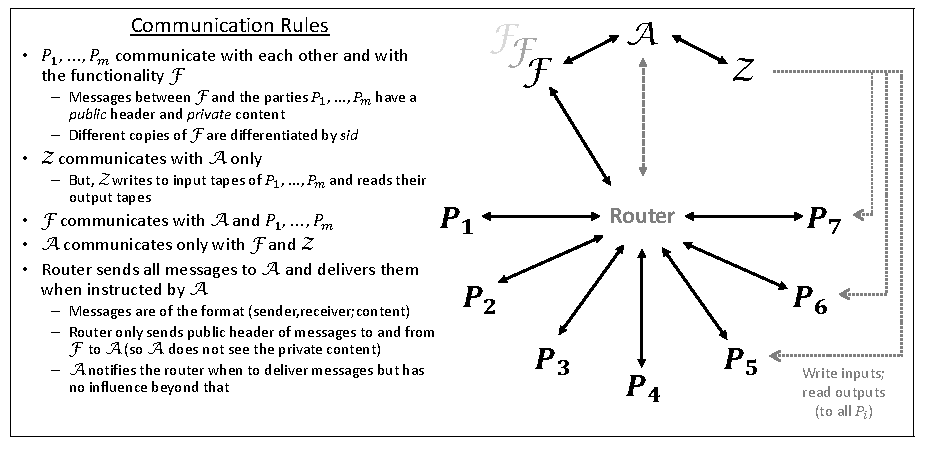
\includegraphics[scale=0.9]{router}
    \caption{The communication model, from the \cite{Canetti_SUC} paper}
    \label{SUC_router}
\end{figure}

The adversary is able to control the router, and thus can delay or block any message. However, the communication is supposed to be authenticated, so the adversary can read the messages between the parties, but it cannot modify them.

Moreover, any communication between a party and the ideal functionality $\Fun$ is comprised of a \texttt{public header} and a \texttt{private content}; the router forwards to the adversary only the \texttt{public header} part of the message.

Formally, the router operates in the following way:
\begin{itemize}
    \item Read any incoming message of the form $(P_i,P_j,x)$ between party $P_i$ and $P_j$; check that $P_i$ is the actual sender, store it and forward the message to $\adv$.
    \item Do the same for any message from/to the functionality, but only forward to $\adv$ the \texttt{public header} part of the content $x$.
    \item When instructed by $\adv$, deliver the message to $P_j$.
\end{itemize}

Notice that in this model of communication we cannot guarantee fairness by definition: all the messages, including the outputs from $\Fun$, may be blocked from the adversary. Moreover, we cannot model local computations (such as encryption) via an ideal functionality, since those calls will be notified to $\adv$ and it might decide to block the output, which is not realistic for a local computation.

Finally, the environment $\zdv$ communicates only with the adversary, and not via the router. However it has access to the input/output tapes of all the parties.

\subsection{Execution and corruptions}

The execution starts from $\zdv$, which is given an input $z\in\bin^\ast$; moreover each machine has the value $\secparam$ in their security parameter tapes.

The environment may at any time write to the input tapes of the parties, read their output tapes or communicate with the adversary.

Then the main loop of execution begins: the adversary reads its incoming communication tape; it can perform any computation and then it may send any of the following messages
\begin{itemize}
    \item Instruct the router to deliver any message; then the receiving party is activated.
    \item Send a direct message to $\Fun$, and activate it.
    \item Send a direct message to $\zdv$, and activate it.
\end{itemize}

Whenever any party is activated, it reads its incoming communication tape, it does whatever computation it needs, and then sends any messages to the router, which will forward all messages to the adversary.

The loop continues until the environment outputs a bit and halts.

Moreover the adversary can corrupt any parties they want, formally by sending a $(\texttt{corrupt}, P_i)$ message through the router. The corrupted party will then follow the adversary instructions, and the environment will be notified.

We will mostly be dealing with \emph{static} corruptions, which means that the adversary can only corrupt a fixed set of parties at the start of the protocol.

There is also the important distinction, as in the stand-alone model, between \emph{semi-honest} and \emph{malicious} adversaries. A semi-honest adversary only gets a read-only access to the internal tapes of a party; this means that the party will follow the prescribed protocol.

In case of a malicious adversary, besides getting access to the internal tapes, the adversary can instruct the router to send any message it wants as the corrupted party, effectively deviating arbitrarily from the protocol.

\subsection{Execution models and security properties}

We are now ready to define real, ideal and hybrid models, from which security definitions and composition theorems will follow. These are special cases of the execution and communication models described above.

\begin{itemize}
    \item The \emph{real model with protocol $\pi$}: there is no ideal functionality $\Fun$, and all the parties communicate with each other following protocol $\pi$. We denote the output bit of the environment $\zdv$ after an execution of $\pi$ with adversary $\adv$ by $\textsc{\scriptsize SUC-REAL}_{\pi,\adv,\zdv}(n,z)$, where $n$ is the security parameter and $z$ is the input of the environment.
    \item The \emph{ideal model with $\Fun$}: all the parties follow a very simple trusted party protocol. In particular, each party sends to the functionality $\Fun$ precisely the value on their input tape, provided by the environment (unless they are corrupted, thus the adversary $\sdv$ can make them send anything to $\Fun$). Moreover they write the message returned by $\Fun$ on their output tapes.
    
    We denote the output of $\zdv$ after this ideal execution with $\Fun$ and adversary $\sdv$ by $\textsc{\scriptsize SUC-IDEAL}_{\Fun,\sdv,\zdv}(n,z)$.
    
    \item The \emph{hybrid model with $\pi$ and $\mathcal G$}: the parties follow protocol $\pi$ and communicate with each other, but may be instructed to communicate with the ideal functionality $\mathcal G$. We denote the output of $\zdv$ after an execution of $\pi$ with ideal calls to $\mathcal G$ against adversary $\adv$ by $\textsc{\scriptsize SUC-HYBRID}^{\mathcal G}_{\pi,\adv,\zdv}(n,z)$
\end{itemize}

We finally give our definition of security, which is very similar to the one used in the stand-alone model, but here we have the environment that acts as a distinguisher.

\begin{definition}
    Let $\pi$ be a protocol and $\mathcal F$ be an ideal functionality. We say that $\pi$ \emph{SUC-securely computes} $\mathcal F$ if for any PPT adversary $\adv$ there exists a PPT simulator $\sdv$ such that for any PPT environment $\zdv$ it holds that
    $$ \{ \textsc{\scriptsize SUC-IDEAL}_{\Fun, \sdv, \zdv} \} \cindist \{ \textsc{\scriptsize SUC-REAL}_{\pi, \adv, \zdv} \}$$
    
    If $\pi$ is a hybrid protocol which uses a functionality $\mathcal G$, we instead say that $\pi$ SUC-securely computes $\Fun$ in the $\mathcal G$-hybrid model if
    $$ \{ \textsc{\scriptsize SUC-IDEAL}_{\Fun, \sdv, \zdv} \} \cindist \{ \textsc{\scriptsize SUC-HYBRID}^{\mathcal G}_{\pi, \adv, \zdv} \}$$
\end{definition}

We observe that for any adversary $\adv$ and environment $\zdv$ there exists an environment $\zdv'$ that includes internally the adversary $\adv$ and communicates with a dummy adversary that simply relays messages between $\zdv'$ and the router. Since the definition quantifies over every adversary and environment, for proving SUC-security it is sufficient to emulate this dummy adversary.

Formally, this dummy adversary $\ddv$ receives messages $(i,j,m)$ from the environment and instructs the router to send message $m$ to $P_j$ from the corrupted $P_i$; moreover, it forwards to $\zdv$ any message received from the router. Finally, it forwards any message from/to the functionality $\Fun$ to/from the environment.

We finally can state the following proposition.
\begin{proposition}
    The protocol $\pi$ SUC-securely computes $\Fun$ if there exists a PPT simulator $\sdv$ such that for any PPT environment $\zdv$ we have 
    $$ \{ \textsc{\scriptsize SUC-IDEAL}_{\Fun, \sdv, \zdv} \} \cindist \{ \textsc{\scriptsize SUC-REAL}_{\pi, \ddv, \zdv} \}$$
\end{proposition}

Exactly as in the stand-alone model and in the full UC framework, protocols can be composed while maintaining SUC-security.

Indeed, if $\pi$ is a protocol for computing $\Fun$ in the $\mathcal G$-hybrid model, and $\rho$ is a protocol for computing $\mathcal G$ (eventually in a $\mathcal H$-hybrid model), we can define the protocol $\pi^\rho$ that computes functionality $\Fun$ in the $\mathcal H$-hybrid model. This is done by replacing the code to calls to $\mathcal G$ with the code for executing $\rho$; we only impose the restriction that different instances of $\rho$ call different instances of $\mathcal H$, if $\rho$ is itself hybrid.

We thus have the following composition theorem.
\begin{theorem}
    Let $\pi$ be a protocol in the $\mathcal G$-hybrid model, and $\rho$ a protocol that SUC-securely computes $\mathcal G$ in the $\mathcal H$-hybrid model. Then for any PPT adversary $\adv$ there exists a PPT simulator $\sdv$ such that for all PPT environments $\zdv$
    $$ \{ \textsc{\scriptsize SUC-HYBRID}^{\mathcal H}_{\pi^{\rho}, \sdv, \zdv} \} \cindist \{ \textsc{\scriptsize SUC-HYBRID}^{\mathcal G}_{\pi, \adv, \zdv} \}$$
    
    In particular, if $\rho$ SUC-securely computes $\mathcal G$, then the protocol $\pi^\rho$ SUC-securely computes the functionality $\Fun$.
\end{theorem}

We conclude this chapter with the main motivation for introducing the SUC framework: it's easier to work with with respect to the full UC framework, but it gives the same security guarantees. The only difference is that not all tasks that can be modelled in UC can also be modelled in SUC.

\begin{theorem}
    Let $\pi$ be a protocol that SUC-securely computes the functionality $\Fun$ in the $\mathcal G$-hybrid model. Then there is a transformation $\phi$ such that the protocol $\phi(\pi)$ UC-realizes the functionality $\phi(\Fun)$ in the $(\phi(\mathcal G), \Fun_{\textsc{AUTH}})$-hybrid model.
\end{theorem}

The details of this transformation and the proof of the theorem, along all other proofs of the theorems in this section, can be found in \cite{Canetti_SUC}.
\part{Oblivious Transfer Protocols}
\chapter{What is Oblivious Transfer?}

\section{Introduction}
Oblivious Transfer is a functionality between two parties, one called \emph{sender} and the other \emph{receiver}. The sender has two messages $m_0,m_1$, while the receiver has a ``choice bit" $\sigma$; at the end of the execution the receiver should know $m_\sigma$ (but nothing about $m_{1-\sigma}$), and the sender shouldn't be able to know $\sigma$.

It is one of the simplest examples of secure multi-party computation, but most importantly any MPC function can be reduced to a composition of many OT protocols. Thus the security and efficency of proposed OT protocols is of great importance.

Efficiency usually is measured in number of rounds, size of the exchanged messages and actual time of computation (or number of operations). Security, as with most MPC protocols, is defined in the UC framework.

The UC framework provides the most security for any protocol, since it gives protection against parallel executions and any kind of composition with other protocols. However full proofs for the case of an adaptive malicious adversary are usually difficult to do and may require some added technicalities to the protocol itself.

Moreover, is has been proved that it's impossible to realize a UC-secure OT protocol in the \emph{plain model}. All protocols thus rely on a Random Oracle or a Common Reference String.

We will define the security of our protocols based on the SUC framework, and in particular will have two parties denoted by S for the sender and R for the receiver.

The full functionality is described below in figure \ref{func_ot_base}.

Formally, any 2-party computation can be modeled by some function $f:\{0,1\}^\ast\times\{0,1\}^\ast\to\{0,1\}^\ast\times\{0,1\}^\ast$. For the Oblivious Transfer protocol one has $f_{OT}((m_0,m_1), \sigma)=(\lambda, m_\sigma)$, where $\lambda$ denotes the empty string.

\begin{figure}
    \begin{center}
            \fbox{\parbox{0.9\linewidth}{\centering
                \textbf{The functionality $\mathcal F_{OT}$}
                \begin{enumerate}
                    \item On input $(\texttt{receive}, sid, \sigma)$ from R, if no message with the same sid has been stored, store $(\texttt{receive}, sid, \sigma)$.
                    \item On input $(\texttt{send}, sid, (m_0, m_1))$ from S, if no message with the same sid has been stored, store $(\texttt{send}, sid, (m_0, m_1))$.
                    \item On input $(\texttt{deliver}, sid)$ from the simulator, if there have been stored both messages $(\texttt{receive}, sid, \sigma)$ and $(\texttt{send}, sid, (m_0, m_1))$, send $(\texttt{output}, sid, m_\sigma)$ to R.
                \end{enumerate}

        }}
    \end{center}
    \caption{The functionality for Oblivious Transfer in the SUC framework}
    \label{func_ot_base}
\end{figure}

HERE: original oblivious transfer protocol. Other things?


\section{Some insecure protocols}

We now describe a couple of OT protocols based on Diffie-Hellman and prove their level of (in)security.

Both protocols will use a fixed prime $p$, and a fixed generator $g$ of $\F_p^\ast$.

Moreover we use a symmetric encryption scheme $\mathcal{E}=(\enc, \dec)$ defined over $(\mathcal{K, M, C})$, with $\mathcal{K}=\F_p^\ast$.

\subsection{Eavesdropper secure}
We describe a possible OT protocol which completely relies on the honesty of both parties.

\begin{figure}
    \myproc{Protocol 1}{
        \textbf{Sender} \> \> \textbf{Receiver} \\
        \text{Input: }(m_0, m_1) \> \> \text{Input: }\sigma \\
        \> \> b_0, b_1 \sample \set{1,\dots, p-1} \\
        \> \> B_i = g^{b_i} \\
        \> \sendmessageleft*{(B_0, B_1)} \> \\
        a_0, a_1 \sample \set{1,\dots, p-1} \> \> \\
        A_i = g^{a_i} \> \> \\
        k_i = B_i^{a_i} \> \> \\
        c_i = \enc_{k_i}(m_i) \> \> \\
        \> \sendmessageright*{(A_0, A_1, c_0, c_1)} \> \\
        \> \> k_\sigma= A_\sigma^{b_\sigma} \\
        \> \> m_\sigma= \dec_{k_\sigma}(c_\sigma) \\
    }
    \caption{The example protocol number 1}
    \label{prot_dummy_1}
\end{figure}

\begin{proposition}
    The protocol 1 does not SUC-securely computes $\Fun_{OT}$ even with a semi-honest adversary.
\end{proposition}

\begin{proof}
    We need to show that there exists an adversary such that for any simulator $\sdv$ there is an environment $\zdv$ which distinguishes the real execution from the ideal one.

    We start by defining the adversary $\adv$, which corrupts the receiver, learns the secret $b_{1-\sigma}$ and then can compute $k_{1-\sigma} = A_{1-\sigma}^{b_{1-\sigma}}$ and finally decrypt $m'=\dec_{k_{1-\sigma}}(c_{1-\sigma})$; then $\adv$ sends back $m'$ to the environment.

    We then define an environment $\zdv$ that checks if $m'=m_{1-\sigma}$ and outputs $1$ if they are equal, $0$ otherwise.

    We claim that no simulator can make that environment output $1$, except with negligible probability, thus the distributions are very distinguishable.

    Indeed the functionality statistically hides the other message $m_{1-\sigma}$ from the simulator, so the best thing the simulator can do is output a random message. \todo{Is it enough?}
\end{proof}

The only property that protocol 1 has is the privacy against external eavesdroppers, since it's basically the execution of an hybrid encryption scheme repeated for two times.


\subsection{Semi-honest}
We now change a little the protocol to make it at least semi-honest. We will prove its security against semi-honest adversaries, but will also show how malicious adversaries can break it.

\begin{figure}
    \myproc{Protocol 2}{
        \textbf{Sender} \> \> \textbf{Receiver} \\
        \text{Input: }(m_0, m_1) \> \> \text{Input: }\sigma \\
        \> \> b_\sigma \sample \set{1,\dots, p-1} \\
        \> \> B_\sigma = g^{b_\sigma} \\
        \> \> B_{1-\sigma} \sample \set{1,\dots, p-1} \\
        \> \sendmessageleft*{(B_0, B_1)} \> \\
        a_0, a_1 \sample \set{1,\dots, p-1} \> \> \\
        A_i = g^{a_i} \> \> \\
        k_i = B_i^{a_i} \> \> \\
        c_i = \enc_{k_i}(m_i) \> \> \\
        \> \sendmessageright*{(A_0, A_1, c_0, c_1)} \> \\
        \> \> k_\sigma= A_\sigma^{b_\sigma} \\
        \> \> m_\sigma= \dec_{k_\sigma}(c_\sigma) \\
    }
    \caption{The example protocol number 2}
    \label{prot_dummy_2}
\end{figure}

\begin{proposition}
    Protocol 2 SUC-securely computes $\Fun_{OT}$ for semi-honest adversaries, if the encryption scheme is \indcpa.
\end{proposition}
\begin{proof}
    Since the corruptions are static, we check the four different cases.

    \textbf{Corrupted sender and honest receiver}: The simulator $\sdv_{S^\ast}$ is described in figure \ref{sim_dummy2_sender}.

    \begin{figure}
        \begin{center}
            \fbox{\parbox{0.9\linewidth}{\centering
                    \textbf{Simulator $\sdv_{S^\ast}$}
                    \begin{itemize}
                        \item Choose $B_0, B_1\sample \set{1,\dots, p-1}$ and notify the environment of the message $(B_0, B_1)$.
                        \item Follow the protocol to compute $A_0,A_1,c_0,c_1$ and notify the environment of such sent message.
                    \end{itemize}
            }}
        \end{center}
        \caption{The simulator for the corrupted sender in protocol 2}
        \label{sim_dummy2_sender}
    \end{figure}

    We show that the transcript provided by the simulator is indistinguishable from a real transcript.

    Indeed the only difference is that in the protocol $B_\sigma = g^{b_\sigma}$; but since $b_\sigma$ is taken uniformly from $\set{1,\dots,p-1}$, also $g^{b_\sigma}$ is distributed uniformly in $\set{1,\dots,p-1}$.

    More formally, if $X_0,X_1$ are two random variables uniformly distributed on $\set{1,\dots,p-1}$, then $(X_0,X_1)$ is identical to both $(X_0, g^{X_1})$ and $(g^{X_0}, X_1)$.

    \textbf{Honest sender and corrupted receiver}: The simulator $\sdv_{R^\ast}$ is described in figure \ref{sim_dummy2_receiver}.

        \begin{figure}
        \begin{center}
            \fbox{\parbox{0.9\linewidth}{\centering
                    \textbf{Simulator $\sdv_{R^\ast}$}
                    \begin{itemize}
                        \item Follow the protocol to compute $B_\sigma$ and $B_{1-\sigma}$, and notify the environment of the sent message $(B_0, B_1)$.
                        \item Query the functionality with input $\sigma$ as the receiver, and get the output $m_\sigma$.
                        \item Follow the protocol to generate $A_0,A_1$, compute the key $k_\sigma$ and the ciphertext $c_\sigma=\enc_{k_\sigma}(m_\sigma)$.
                        \item Generate a random key $k_{1-\sigma}\sample\mathcal{K}$ and compute $c_{1-\sigma}=\enc_{k_{1-\sigma}}(0)$.
                        \item Notify the environment of the received message $(A_0, A_1, c_0, c_1)$.
                    \end{itemize}
            }}
        \end{center}
    \caption{The simulator for the corrupted receiver in protocol 2}
    \label{sim_dummy2_receiver}
    \end{figure}

    We will now show that the environment cannot distinguish the simulator from a real transcript.

    We use an intermediate simulator $\sdv'$ which differs from $\sdv_{R^\ast}$ only in that $c_{1-\sigma}=\enc_{k_{1-\sigma}}(m_{1-\sigma})$ (but the key is still random).

    \begin{itemize}
        \item \textit{Indistinguishability of $\sdv_{R^\ast}$ and $\sdv'$}.\\
        If an environment $\zdv$ can distinguish the simulators, then we can use it to break $\indcpa$.\todo{Formalize this: to get an oracle we need to cheat with randomness}
        \item \textit{Indistinguishability of $\sdv'$ and a real execution}.\\
        Suppose we have an environment $\zdv$ that is able to distinguish; then we can use it to break the decisional Diffie-Hellman assumption.\\
        We construct the following distinguisher $\ddv$, which takes as input any triple $(g^a,g^b,g^c)$. Internally, $\ddv$ makes the simulator $\sdv'$ generate $B_{1-\sigma}=g^b$ and $a_{1-\sigma}=a$; then sets $k_{1-\sigma}=g^c$.\\
        Since $\zdv$ can distinguish the ``correct" key from a random one, it will also distinguish a random $c$ from the value $ab$.\todo{Write precise probabilities, check which properties of encryption scheme are used}
    \end{itemize}

    In conclusion, the environment cannot distinguish the simulator from a real execution.

    \textbf{Corrupted sender and corrupted receiver}: The simulator can just execute the protocol with the input it knows.

    \textbf{Honest sender and honest receiver}: Here the simulator runs the protocol with inputs $(m_0,m_1)=(0,0)$ and $\sigma=1$.

    Using what is proved above, we can construct a series of intermediate simulators from the real execution to the one with fixed inputs.
\end{proof}

We have thus proved semi-honest security for protocol 2, which for some kind of tasks might be enough. However, we see that a malicious receiver can easily learn both messages.

It is sufficient to sample a random $b\sample\set{1,\dots,p-1}$, then compute $B_{1-\sigma}=g^b$ and use this secret value of $b$ to decrypt $c_{1-\sigma}$ by computing the other key $k_{1-\sigma}=A_{1-\sigma}^b$.

This is an example of why we are looking for UC-secure protocols with malicious adversaries.



\section{Chou and Orlandi OT}

We will analyze an important OT protocol of the recent years; it is one of the most efficient ones, but its security is based on classical DH (over elliptic curves) and cannot be proven to be fully UC-secure.

The core of the protocol is described in figure \ref{prot_CO}. The function $H$ is modeled as a random oracle, and the protocol is implemented with Edwards curves.

\begin{figure}
    \myproc{Protocol $\Pi_{CO}$}{
        \textbf{Sender} \> \> \textbf{Receiver} \\
        \text{Input: }(m_0, m_1) \> \> \text{Input: }\sigma \\
        a \sample \set{0,\dots, p-1} \> \>b \sample \set{0,\dots, p-1} \\
        A = g^a \> \> \\
        \> \sendmessageright*{A} \> \\
        \> \> B = A^\sigma\cdot g^b \\
        \> \sendmessageleft*{B} \> \\
        k_i = H((B/ A^{i})^a) \> \> k_\sigma = H(A^b) \\
        c_i = k_i \oplus m_i \> \> \\
        \> \sendmessageright*{(c_0, c_1)} \> \\
        \> \> m_\sigma= k_\sigma \oplus c_\sigma \\
    }
    \caption{The Simplest OT protocol by Chou and Orlandi}
    \label{prot_CO}
\end{figure}


\section{Security in the algebraic group model}

One possible solution to make the Chou and Orlandi protocol secure is to change the definition of what ``secure" means; in particular we can limit the adversary to behave \emph{algebraically} and then be able to complete the proofs.

In the Algebraic Group Model (AGM in short) every machine that outputs a group element $g\in\mathbb G$ must be able to ``explain" it, i. e. output also a representation vector $(x_1,\dots,x_n)$ such that $g=\prod_{i=1}^n g_i^{x_i}$, where the $g_i$s are called a \emph{base} and are the group element already seen by that party.

The approach of combining the AGM and the UC framework has been studied in \cite{AGM_UC}; we will follow their exposition, summarizing the most important points.

\subsection{Defining AGM-UC}

We will keep using the simplified UC framework, with a fixed number of parties for every protocol.

The setting involves a group $\mathbb G$ of order $p$, with known generator $g$; we collect those parameters in $\mathcal G=(\mathbb G, g, p)$.

\begin{definition}
    Suppose a protocol $\pi$ uses the group $\mathcal G$. A pair of environment $\edv$ and adversary $\adv$ is said $(\mathcal G,\pi)$-algebraic if whenever $\adv$ sends a $(\texttt{backdoor}, m)$ message to a party and $m$ contains an element $h\in\mathbb G$, then it must provide (to a special ``algebraic tape") an algebraic representation $X$ of $h$, which is a list $X=[(g_1,x_1),\dots,(g_k,x_k)]$ such that $h=\prod_{i=1}^kg_i^{x_i}$ and $g_i$ are group elements already seen by $\adv$ or $\edv$ in the execution of $\pi$.
\end{definition}

Now we are able to define simulation:

\begin{definition}
    Suppose protocols $\pi$ and $\phi$ involve the same group $\mathcal G$. We say that $\pi$ \emph{$\mathcal G$-AGM emulates} $\phi$ if for any adversary $\adv$ there is a simulator $\sdv$ such that for any environment $\edv$ with $(\edv,\adv)$ that is $(\mathcal G, \pi)$-algebraic we have that also $(\edv,\sdv)$ is $(\mathcal G, \phi)$-algebraic and
    $$EXEC_{\phi,\sdv,\edv} \cindist EXEC_{\pi,\adv,\edv}$$
\end{definition}

We can use dummy adversaries also in this algebraic setting; we need only to pay attention to the algebraic representations that the environment send to the adversary, because we don't want to forward them to the actual protocol.

\begin{definition}
    Suppose the protocol $\pi$ involves $\mathcal G$. An adversary $\ddv$ is \emph{$(\mathcal G, \pi)$-algebraically dummy} if it only forwards messages in this way:
    \begin{itemize}
        \item For any received message of the type $(\texttt{backdoor},m)$ from a party $ID$, sends $(\texttt{backdoor},(ID, m))$ to $\edv$.
        \item For any $(\texttt{input},(ID, m))$ from $\edv$, it sends $(\texttt{input}, m')$ to ID, where $m'$ is equal to $m$, but without all algebraic representations $X$ of elements $h\in\mathbb G$ which are inside $m$.
    \end{itemize}
\end{definition}

With this definition of dummy adversary we then have the theorem.

\begin{theorem}
    Suppose protocols $\pi$ and $\phi$ involve group $\mathcal G$. Then $\pi$ $\mathcal G$-AGM emulates $\phi$ if and only if $\pi$ $\mathcal G$-AGM emulates $\phi$ with respect to the dummy adversary.
\end{theorem}

Observe also that since the dummy adversary doesn't output any algebraic representation, they must all come from the environment.

We then have the composition theorem, but need to pay attention to the different bases the adversary can use.\todo{maybe write this}

\subsection{Proof of AGM-UC security of Chou and Orlandi}

The algebraic model is a key tool for proving UC security for the \emph{simplest OT} protocol. The authors use the algebraic behaviour of the adversary both for explaining the parties' state after adaptive corruptions and for extracting the input bit of a corrupt receiver.

We will only give a sketch of the proof in the case of static corruptions.

We use the protocol in figure \ref{prot_CO}, with the functionality presented in figure \ref{func_ot_agm}.

\begin{figure}
    \begin{center}
        \fbox{\parbox{0.9\linewidth}{\centering
                \textbf{The functionality $\mathcal F_{OT}$}
                \begin{itemize}
                    \item On input $(\texttt{receive}, sid, \sigma)$ from R or $\sdv$, if no message with the same sid has been stored, store $(\texttt{receive}, sid, \sigma)$ and notify $\sdv$.
                    \item On input $(\texttt{send}, sid, (m_0, m_1))$ from S or $\sdv$, if no message with the same sid has been stored, store $(\texttt{send}, sid, (m_0, m_1))$ and notify $\sdv$.
                    \item On input $(\texttt{deliver}, sid, R)$ from the simulator, if there have been stored both messages $(\texttt{receive}, sid, \sigma)$ and $(\texttt{send}, sid, (m_0, m_1))$, send $(\texttt{output}, sid, m_\sigma)$ to R; otherwise output $\bot$ to $\sdv$.
                    \item On input $(\texttt{deliver}, sid, S)$ from the simulator, if it was previously output $(\texttt{output}, sid, m_\sigma)$, then send $(\texttt{output}, sid)$ to S; otherwise output $\bot$ to $\sdv$.
                \end{itemize}

        }}
    \end{center}
    \caption{The functionality for Oblivious Transfer in the AGM-UC framework}
    \label{func_ot_agm}
\end{figure}

\begin{theorem}
    The protocol $\Pi_{CO}$ AGM-realizes the functionality $\Fun_{OT}$ in the $\Fun_{RO}$-hybrid model under static corruptions.
\end{theorem}
\begin{proof}
    We construct a simulator $\sdv$ for the dummy algebraic adversary in each of the four corruption cases. By definition, this means that all group elements output by $\edv$ to $\sdv$ must have a representation.

    \textbf{Corrupted sender and corrupted receiver}: Here there is nothing to simulate.

    \textbf{Honest sender and honest receiver}:

    \textbf{Corrupted sender and honest receiver}: When $\sdv$ receives $A$ from the environment, it also learns the value $a$ such that $A=g^a$.
    The simulator then chooses a random $b$, computes $B=g^b$, and sends it back to $\edv$.

    Then it computes the key $k=H(A^b)$. When the environment sends any $(c_0,c_1)$, the simulator sends $(c_0\oplus k, c_1\oplus k)$ to the trusted party and makes it deliver to the honest receiver.

    This simulates correctly since the output of the receiver is identical in both the ideal and the real execution; moreover the distributions $g^{a\sigma+b}$ and $g^b$ are identical, so the environment cannot distinguish between the case $\sigma=0$ and $\sigma=1$.

    \textbf{Honest sender and corrupted receiver}: The simulator samples $a$, computes $A=g^a$ and sends it to the environment, which responds with an arbitrary element $B$; since $\edv$ is algebraic, it must also output a representation $B=A^x g^y$.

    If $x\in\{0,1\}$, the simulator queries the functionality with this bit, retrieves $m_x$, chooses a random $m_{1-x}$ and finally computes $k_i,c_i$ as specified in the protocol. If $x\not\in\{0,1\}$, the simulator chooses both $m_0$ and $m_1$ as random.

    The simulator also runs the random oracle, and counts the queries the enviroment makes to it. Moreover, if $x\in\{0,1\}$ and $\edv$ queries for both $B^a$ and $B^a\cdot g^{-a^2}$, of if $x\not\in\{0,1\}$ and $\edv$ queries at least one of $B^a$ or $B^a\cdot g^{-a^2}$, then $\sdv$ aborts.

    \textit{Claim}: $\sdv$ aborts with negligible probability if the discrete logarithm is hard.\todo{Make quantitative with number of queries}

    Suppose we want to solve the discrete logarithm problem $A=g^z$, using $\edv$ as an oracle. We feed $\edv$ the element $A$ as coming from the simulator.
    \begin{itemize}
        \item Case $x\not\in\{0,1\}$. Suppose $\edv$ queries $B^z$; being algebraic, it must know a representation $B^z=A^sg^t$. But this means that $g^{z^2x+zy}=(A^xg^y)^z=B^z=g^{sz+t}$, i.e. $$z^2x+z(y-s)-t\equiv 0\pmod p$$ from which we can compute $z$. In the other case we have that $B^zg^{-z^2}=A^sg^t$, for which the equation is $z^2(x-1)+zy\equiv sz+t\pmod p$, which also has a solution.
        \item Case $x=0$. The environment has queried $B^zg^{-z^2}$, for which it knows a representation $A^sg^t$. Then it gets the equation $zy-z^2\equiv sz+t\pmod p$, which has a solution.
        \item Case $x=1$. The environment has queried $B^z$, and represents it as $A^sg^t$. Then the equation is $z^2+zy\equiv sz+t\pmod p$, which also has a solution.
    \end{itemize}

    This concludes the proof since if the simulator doesn't abort, the simulation is perfect, given that the keys queried from the random oracle statistically hide the messages. Finally we observe that all the simulators we have constructed are algebraic themselves.
\end{proof}

\chapter{Analysis of isogeny OT protocols}

\section{An overview of proposed protocols}
In this section we briefly discuss the security levels of some isogeny-based OT protocols that have been proposed in the last few years.

\begin{itemize}
    \item \cite{Barreto, Branco}: in the first paper by Barreto et al., they introduce a protocol based on SIDH; it constructs a SIDH public key and creates a second ``fake" public key by perturbing the public torsion points. Its security is thus based on the indistinguishability of $(\phi(P),\phi(Q))$ and $(\phi(P)+U,\phi(Q)+V)$, where $U,V$ are random $E[\ell^e]$ torsion points and $\{P,Q\}$ is the SIDH basis of $E_0[\ell^e]$.\\
    Based on this indistinguishability assumption, Branco et al. build an implementation of their proposed OT protocol framework. The resulting OT protocol has four rounds and is proved to be UC-secure against malicious adversaries.\\
    However, we notice that Barreto et al. say they have identified some problems in the security of their protocol (which is not even made in the UC framework), so also the derived protocol by Branco et al. could have problems.
    
    \item \cite{Vitse}: the author constructs a SIDH-based protocol using an exponentiation-only construction; in Diffie-Hellman terms this means that the receiver gets the public keys $g^{a_0},g^{a_1}$, sends back $\left(g^{a_\sigma}\right)^b$ and receives $g^{a_\sigma\cdot b\cdot a_i^{-1}}$ as possible keys. In the SIDH context, the author uses dual isogenies and additional helper points to achieve this construction.\\
    The resulting OT protocol has three rounds, and is proved to be secure against malicious adversaries but using a game-based definition of security for OT. Moreover, the author introduces additional hardness assumptions to conclude her proofs.
    
    \item \cite{dSG_Orsini}: the authors introduce the concept of \emph{masking}, which generalizes the one of hard homogeneous spaces; this allows them to create masks from both SIDH and CSIDH.\\
    They then construct a couple of OT protocols, one with two rounds and the other with three rounds, and prove the UC-security of both of them against semi-honest adversaries.\\
    Moreover, the authors prove that their two-round protocol can be extended to be secure against malicious adversaries using a transformation by D{\"o}ttling \cite{Dottling}.
    
    \item \cite{Alamati}: the authors introduce a new framework based on group actions, from which they derive new cryptographic primitives based on CSIDH. In particular, they construct a ``dual-mode encryption scheme"; this allows them to use the framework by Peikert et al. \cite{PVW} to produce an OT protocol that is UC-secure against malicious adversaries.\\
    The resulting protocols has only two rounds, but the PVW framework transmits single bits, so for sending $n$-bit messages we need to send $O(n)$ public keys and compute $O(n)$ isogenies.
\end{itemize}

In conclusion, there doesn't seem to exist a protocol that is both \emph{efficient} (i.e. two rounds with constant computations) and UC-secure against \emph{malicious} adversaries.

\subsection{A CSIDH based protocol}
One more OT protocol based on isogenies is the one proposed by Lai, Galbraith and de Saint Guilhem in \cite{Lai_twists}; it works in the CSIDH setting, and makes a clever use of the twisting operation.

The protocol written in Figure \ref{prot_twist} is two-round and uses a trusted setup curve $E$. It is only proved to be semi-honest secure in the UC framework, but there is a version with three rounds that is secure against static malicious corruptions.

The third round in the malicious secure version is added as a ``proof of decryption", which makes possible to extract the input of a malicious receiver. This three-round maliciously secure protocol adds many operations and is much less readable; most of the added operations deal with the difficulty of extracting corrupted inputs in the UC proof, thus it seems very artificial.

\begin{figure}
    \myproc{Protocol $\Pi_{tw}$}{
        \textbf{Sender} \> \> \textbf{Receiver} \\
        \text{Input: }(m_0, m_1) \> \> \text{Input: }\sigma \\
        s \sample Cl \> \> r \sample Cl \\
        A = s\star E \> \>  C = r\star E \\
        \> \> \text{if } \sigma=1: C=C^t \\
        \> \sendmessageleft*{C} \> \\
        k_0 = H(s\star C) \> \>\\
        k_1 = H(s\star C^t) \> \>\\
        c_i = \enc_{k_i}(m_i) \> \> \\
        \> \sendmessageright*{A, (c_0, c_1)} \> \\
        \> \> k_\sigma = H(r\star A) \\
        \> \> m_\sigma= \dec_{k_\sigma}(c_\sigma) \\
    }
    \caption{The twist OT protocol by Lai et al.}
    \label{prot_twist}
\end{figure}


\section{Defining the ``explicit isogeny model"}
The main idea of this chapter is that we want to use the Algebraic Group Model (AGM) in the isogeny setting, since it's very helpful with proofs. However, we don't want to restrict too much the power of the adversary. We will thus define a new model, analogous to AGM; in Section \ref{section_EIgeneral} we will show some evidence on the fact that our model could be equivalent to the plain model.

\begin{definition}
    We say that a Turing machine $\adv$ \emph{uses Explicit Isogenies} (EI) if whenever it outputs a supersingular elliptic curve $E$, it also outputs a computable isogeny $\phi:E_1\to E$, where $E_1$ is a curve that it has already seen.
\end{definition}

Here by ``computable" we mean with smooth degree, and given as the composition of small degree isogenies.

We also need to account for the CSIDH framework, with curves over $\F_p$ and a fixed order $\Oc=\End(E_0)$ inside $K=\Q(\sqrt{-p})$.

In this setting, the EI assumption should translate to the adversary being able to output a (smooth) class group element for every supersingular curve it outputs, i.e. always explain $E=x\star E_i$ (or $E_i^t$) for any $E_i$ that it has already seen.

This motivates the following definition.

\begin{definition}
    We say that a Turing machine $\adv$ \emph{uses CM-explicit isogenies} if whenever it outputs a supersingular elliptic curve $E/\F_p$, it also outputs a smooth norm ideal $\mathfrak a\in Cl(\Oc)$ such that $E=\mathfrak a\star E_1$, where $E_1$ is a curve that it has already seen, or its twist.
\end{definition}

We then define what we mean by emulation and realization in this setting, which simply breaks down to the adversary and environment using explicit isogenies.

\begin{definition}
        Given a protocol $\pi$ and a functionality $\Fun$, we say that $\pi$ \emph{(CM)EI-realizes} $\Fun$ if for any adversary $\adv$ there is a simulator $\sdv$ such that for any environment $\edv$ with $(\edv,\adv)$ that use (CM-)explicit isogenies we have that
    $$\{\textsc{\scriptsize IDEAL}_{\Fun,\sdv,\edv} \} \cindist \{\textsc{\scriptsize REAL}_{\pi,\adv,\edv} \}$$
\end{definition}


\section{Proving security in the EI model}
We now prove the security of the two-round twist protocol described in Figure \ref{prot_twist}, using an encryption scheme $\edv=(\kgen, \enc, \dec)$.

The precise result is the following.

\begin{theorem}
    The protocol $\Pi_{tw}$ CMEI-realizes the functionality $\Fun_{OT}$, if the encryption scheme $\edv$ is \indcpa secure.
\end{theorem}
\begin{proof}
    \textbf{Honest sender and corrupted receiver.} The simulator is defined by the following instructions:
    \begin{enumerate}
        \item Backdoors the trusted setup and sets the curve $E=t\star E_0$, with a randomly sampled $t\in Cl(\Oc)$.
        \item Sets its public key as the honest sender $A=s\star E$.
        \item When receiving the curve $C$ from the adversary, there is also an explanation $C=x\star E_R$, with $E_R=E_0,E$ or $E^t$. If $E_R=E$ it sets $\sigma=0$, if $E_R=E^t$ it sets $\sigma=1$, otherwise it sets $\sigma=-1$. If $\sigma\neq -1$, the simulator queries the functionality and gets the message $m_\sigma$.
        \item The simulator samples two random keys $k_i\xleftarrow{}\kgen()$ and begins to monitor the random oracle queries from the adversary for the following values:
        \begin{itemize}
            \item Query is $s\star C$; if $\sigma\neq0$ aborts, otherwise returns $k_0$.
            \item Query is $s\star C^t$; if $\sigma\neq1$ aborts, otherwise returns $k_1$.
        \end{itemize}
        \item The simulator sets any $m_i$ that it doesn't know to $0$ (i.e. $m_{1-\sigma}$ if $\sigma\in\bin$, both $m_0,m_1$ otherwise); then it computes $c_i=\enc_{k_i}(m_i)$.
        \item Finally $\sdv$ sends $A,c_0,c_1$ to the adversary.
    \end{enumerate}
    
    Let $A$ be the event that $\sdv$ aborts, and let $\zdv_\sdv$ denote $\textsc{\scriptsize IDEAL}_{\Fun,\sdv,\zdv}$, while $\zdv_\pi$ denote $\textsc{\scriptsize REAL}_{\pi,\adv,\zdv}$. Then we have
    \begin{align*}
         & \left|\prob{\zdv_\sdv=1}-\prob{\zdv_\pi=1}\right| =\\
        = & \left|\condprob{\zdv_\sdv=1}{A}\cdot\prob{A} + \condprob{\zdv_\sdv=1}{\neg A}\cdot\prob{\neg A} -\right.\\
        & \left.- \condprob{\zdv_\pi=1}{A}\cdot\prob{A} - \condprob{\zdv_\pi=1}{\neg A}\cdot\prob{\neg A}\right| \\
        \le & \left| \condprob{\zdv_\sdv=1}{A} - \condprob{\zdv_\pi=1}{A}\right|\cdot\prob{A}  +\\
         &+ \left| \condprob{\zdv_\sdv=1}{\neg A} - \condprob{\zdv_\pi=1}{\neg A}\right|\cdot\prob{\neg A} \le \\
        \le & \prob{A} + \left| \condprob{\zdv_\sdv=1}{\neg A} - \condprob{\zdv_\pi=1}{\neg A}\right|
    \end{align*}

    The theorem will then follow from the fact that both quantities are negligible. Indeed if $\sdv$ aborts, then we can solve a CSIDH problem, while if $\zdv$ can distinguish we can break the $\indcpa$ property of the encryption scheme.
    
    Indeed, suppose that $\sdv$ does not abort; then we can construct an adversary $\ddv$ for the $\indcpa$ game similarly to what we did in Section \ref{section_dummy}: internally $\ddv$ runs $\zdv$ against $\sdv$, but stopping the execution before the simulator computes $c_{1-\sigma}$.
    
    Then $\ddv$ takes the input $(m_0,m_1)$ for the honest sender, and sends to the $\indcpa$ oracle the pair of messages $(0,m_{1-\sigma})$, which returns a ciphertext $c$; at this points $\ddv$ resumes the execution, but puts $c_{1-\sigma}=c$. Finally $\ddv$ outputs whatever $\zdv$ outputs.
    
    Notice that when the bit $b$ of the $\indcpa$ oracle is $1$, $\ddv$ runs a perfect emulation of the real protocol, while if $b=0$, $\ddv$ is running $\sdv$.
    
    This means that
    
    \begin{align*}
    \advantage{\indcpa}{\ddv,\edv}[] &= \left| \condprob{\ddv=1}{b=0} -  \condprob{\ddv=1}{b=1}\right|\\
    & = \left| \condprob{\zdv_\sdv=1}{\neg A} - \condprob{\zdv_\pi=1}{\neg A} \right|.
    \end{align*}
    In particular $\zdv$ cannot distinguish $\sdv$ and the real world if the encryption scheme $\edv$ is $\indcpa$, in the case that $\sdv$ doesn't abort.    
    
    Let's now estimate the probability of $\sdv$ aborting. Suppose then that we have a CSIDH problem $E_1=a\star E_0$ we want to solve. We create two possible solvers for this problem:
    \begin{itemize}
        \item Algorithm $\ddv_1$ will run $\sdv$ with $E_1$ as the trusted setup; then it will check if it can compute $a$ from the queries and explanations that $\zdv$ makes to the random oracle.
        \item Algorithm $\ddv_2$ will run $\sdv$ with $b\star E_0$ as a trusted setup and $b\star E_1$ as the public key of the sender; then it will check queries to compute a value $a'$ such that $a'\star(b\star E_0)=b\star E_1$, which means $a'=a$.
    \end{itemize}
    
    In Table \ref{tab_dlogs} we show how $\ddv_1$ and $\ddv_2$ can compute the solutions from the query. The rows are indexed by the explanation of the curve $C$ and the query, while the columns are the explanation of the query.
    
    \begin{table}[]
        \centering
        \resizebox{\columnwidth}{!}{%
        \begin{tabular}{c|ccccc}
            & $y\star E_0$ & $y\star E$ & $y\star E^t$ & $y\star A$ & $y\star A^t$ \\
            \hline
            $C=x\star E_0$, $s\star C$ & $s=yx^{-1}$ & $s=ytx^{-1}$ & $s=yt^{-1}x^{-1}$ & $t=xy^{-1}$ & $s^2=x^{-1}t^{-1}$ \\ 
            $C=x\star E_0$, $s\star C^t$ & $s=yx$ & $s=ytx$ & $s=yt^{-1}x$ & $t=x^{-1}y^{-1}$ & $s^2=xt^{-1}$ \\
            $C=x\star E$, $s\star C^t$ & $s=xyt$ & $s=xyt^2$ & $s=xy$ & $t=x^{-1}y^{-1}$ & $s^2=xy$ \\
            $C=x\star E^t$, $s\star C$ & $s=x^{-1}yt$ & $s=x^{-1}yt^2$ & $s=x^{-1}y$ & $t=xy^{-1}$ & $s^2=x^{-1}y$ \\
        \end{tabular}
        }
        \caption{The computable solutions to the CSIDH problem}
        \label{tab_dlogs}
    \end{table}
    
    We now compute $\prob{\sdv\text{ aborts}}$ and estimate it with the advantages of $\ddv_1,\ddv_2$ for the CSIDH problem.
    
    Let $T_1$ be the event that $\zdv$ makes one of the ``forbidden" queries and explains it as $y\star A$ (so $t$ can be computed); let $T_2$ be the event that a forbidden query is made and is explained differently from $y\star A$ (in which case $s$ can be computed).
    
    Notice that $\sdv$ only aborts when a forbidden query is made, so we have $A=T_1\cup T_2$ and in particular $\prob{A}=\prob{T_1}+\prob{T_2}$.
    
    Moreover $\ddv_i$ wins with probability $1$ if event $T_i$ happens, so we have that $$\advantage{CSIDH}{\ddv_i}[]\ge 1\cdot \prob{T_i} + \frac{1}{\# Cl(\Oc)}\prob{\neg T_i}\ge\prob{T_i}$$
    
    In particular we get that $\prob{\sdv\text{ aborts}} \le \advantage{CSIDH}{\ddv_0}[] + \advantage{CSIDH}{\ddv_1}[]$, from which we finally get that
    $$ \left|\prob{\zdv_\sdv=1}-\prob{\zdv_\pi=1}\right| \le \advantage{\indcpa}{\ddv}[] + \advantage{CSIDH}{\ddv_0}[] + \advantage{CSIDH}{\ddv_1}[], $$
    which proves indistinguishability, provided that the encryption scheme is $\indcpa$ and the CSIDH problem is hard.
    
\end{proof}


\section{The generality of EI model}\label{section_EIgeneral}

The EI model limits the capabilities of the adversary, so it may seem that it's less expressive than the plain model of UC security. However, there is a strong evidence suggesting that any PPT adversary behaves like in the explicit isogeny model; in particular, it's ``hard" to sample random supersingular curves without taking a random isogeny walk from another known curve.

Indeed one of the main open problems in isogeny crypto is that of ``hashing-to-curve", which can be roughly stated as follows.
\begin{problem}[Informal]\label{problem_sampling}
    Find an efficient sampling algorithm $E\sample SS_p$, from which computing $\End(E)$ is still hard.
\end{problem}

We identify the main focal points for a complete analysis of the EI model in the following two claims:

\begin{claim}\label{claim_CMEI}
    The EI model and the CMEI model are equivalent.
\end{claim}

\begin{claim}\label{claim_EIUC}
    The EI model is equivalent to the plain UC model.
\end{claim}

The first claim concerns with the relationship between the generic isogeny finding problem and the CSIDH problem; the second deals with some variation of the problem of sampling.

The paper by Castryck et al. \cite{CSIDH_EndRing} is mostly about the first claim, but also makes important considerations about the second. Indeed, they study the paper by Br{\"o}ker \cite{Broker} which is the only known way to generate random supersingular curves besides walking in the isogeny graph; Br{\"o}ker uses the theory of complex multiplication, but the authors conclude that for those curves it's easy to find an isogeny to a base known curve.

Their other main result is an algorithm that given two curves $E_1,E_2$ over $\F_p$ and their full endomorphism rings outputs a class group element $\mathfrak{a}$ such that $\mathfrak{a}\cdot E_1=E_2$. The problem is that this ideal usually doesn't have a smooth norm, so its action cannot be efficiently computed; in order to smoothen the norm we need to find relations in $Cl(\Oc)$ and then run lattice reduction algorithms, which greatly increase complexity.

The new article by Wesolowski \cite{Weso_CSIDH} seems to imply that the CSIDH problem is actually equivalent to \texttt{EndRing}, by giving a polynomial time reduction.

However, these works cannot be directly translated into a proof of the first claim, since the main problem there is translating an $\F_{p^2}$ isogeny $\phi: E_1\to E_2$ into a smooth ideal. If the full $\End(E_1)$ is known (for example if $E_1$ is $y^2=x^3+x$), we could use both results to get an element of $Cl(\Oc)$; but in general we cannot hope to know $\End(E_1)$, for example if $E_1$ is given to us from another party.

This means that proving Claim \ref{claim_CMEI} is as of now an open problem, and probably a hard one. It's also possible that we did not choose the optimal definition for our (CM)EI models.

Claim \ref{claim_EIUC} is instead related to Problem \ref{problem_sampling}, which is considered an open problem in the field of isogeny-based cryptography, as stated also in \cite{CSIDH_EndRing}. It's slowly becoming a common belief among isogenists that this problem might be difficult to solve.

We are thus very tempted to pose the following assumption.

\begin{assumption}
    Sampling a supersingular curve $E$ without learning a path from a known curve $E_0$ is hard.
\end{assumption}

This is because if the assumption holds, then Claim \ref{claim_EIUC} seem to follow almost ``by definition", and thus we have gained ``for free" an effective tool for analysing security of isogeny-based MPC protocol.

It is important to know that the posed assumption is not equivalent to Problem \ref{problem_sampling}: knowing an isogeny $\pi: E_0\to E$ is equivalent to knowing $\End(E)$ only if we can compute $\End(E_0)$ (for example if it is $y^2=x^3+x$), but in an interactive protocol a party can receive a supersingular curve from other parties, without being able to know its endomorphism ring.

The assumption is thus trying to model exactly the multi-party computation setting, by forcing any party to generate new curves only by walking in the isogeny graph, starting from curves that have been sent to him.

Notice that if instead the assumption doesn't hold and parties have other ways to generate supersingular curves, then the EI model is actually less expressive than the plain model, in the same way that the AGM denies the sampling of random group elements, which is a very easy operation both for finite fields and for elliptic curves.

However, an efficient sampling algorithm will remove the need of trusted setups of curves, like in our analyzed protocol: instead of being generated by some trusted third party, the common parameter $E$ could be independently computed by both parties only using a common seed.

The conclusion of this chapter is that depending on the hardness of Problem \ref{problem_sampling} we can either have a strong tool for proving security of more efficient protocols, or the removal of trusted setups.






\backmatter
\chapter*{Conclusion}
\addcontentsline{toc}{chapter}{Conclusion}

In this thesis we have introduced a new model for UC-security proofs of isogeny-based protocols; we were inspired by the Algebraic Group Model, which allowed for a security proof of the Chou and Orlandi ``simplest OT" protocol, whose proof instead had important problems.

Indeed, one of the things that we point out is that proofs of UC-security are \emph{hard}, and it's easy to miss some details that might make the proof invalid. In particular, it's very important to carefully design the ideal functionality in order to make it match precisely the security guarantees that we wanted.

For oblivious transfer in particular we have some choices to make, and our protocols will need to account for them: do we let the sender know if the receiver has already submitted its choice bit? Do we let the sender know when the receiver gets his message?\\
We say that $\Fun_{OT}$ should send an empty output message to the sender, but this implies being able to extract the input from the choice of the receiver's public key.

We thus introduce the \emph{Explicit Isogeny} model, that mimics the AGM but for isogeny-based protocols. In particular, we study the OT protocol by Lai et al., proving its security in the EI model even without the additional third round that serves as ``proof of decryption": using the additional isogeny given by the EI model we are indeed able to extract the corrupted receiver's input directly from his public key.

An interesting future work would be trying to prove security of other isogeny-based MPC protocols in the EI model, starting from the already semi-honest OT protocol by de Saint Guilhem et al.; there are also other proposed OT protocols, based both on SIDH and CSIDH, that have not been analyzed at all in the UC framework.

Another work that could be done on those other protocol, starting from the one that we studied in this thesis, is to benchmark the performances of the original protocol and the (possibly more efficient) version that is secure in the EI model. This requires both implementing said protocols and finding the correct more efficient variant, two highly non-trivial tasks.

From a theoretical point of view, we think that future analysis could be made on our last two claims, which are also very correlated to important problems in isogeny-based cryptography: the unification of the SIDH and CSIDH world, and the ``hash-to-curve" problem.

The truth of the first claim would mean the convenience of using either isogeny walks or elements of the class group based on the context, but resulting in the same security guarantees. The truth of the second claim would result in automatically proving full UC-security, while being able to use the power of the EI model for analyzing more compressed protocols.

Even an efficient solution of the sampling problem would be a great result for isogeny-based cryptography, because even if it weakens the EI model, it would remove the requirement of many trusted setups. Thus we think that the sampling problem is really worth more study.

We conclude by saying that our EI model could really be a key tool for having more efficient MPC protocols, while still achieving full UC-security.
%\include{./Chapters/grazie}

%\nocite{*}
\bibliography{Bibliografia}
\bibliographystyle{alpha}


\end{document}
